\documentclass[12pt,pdflatex,authoryear]{elsarticle}

%%%%%%%%%%%%%%%%%%%%%%%%%%%%%%%%%%%%%%%%%%%%%%%%%%
%%%%%%%%%%%%%%%%%%%% PREAMBLE %%%%%%%%%%%%%%%%%%%%
%%%%%%%%%%%%%%%%%%%%%%%%%%%%%%%%%%%%%%%%%%%%%%%%%%


% -------------------- defaults -------------------- %
% load lots o' packages

% references
\usepackage{natbib}

% Fonts
\usepackage[default,oldstyle,scale=0.95]{opensans}
\usepackage[T1]{fontenc}
\usepackage{ae}

% to colorize links in document. See color specification below
\usepackage[pdftex,hyperref,x11names]{xcolor}
% load the hyper-references package and set document info
\usepackage[pdftex]{hyperref}

% Generate some fake text

\usepackage{blindtext}

% layout control
\usepackage{geometry}
\geometry{verbose,tmargin=1.25in,bmargin=1.25in,lmargin=1.1in,rmargin=1.1in}
\usepackage{parallel}
\usepackage{parcolumns}
\usepackage{fancyhdr}

% math typesetting
\usepackage{array}
\usepackage{amsmath}
\usepackage{amssymb}
\usepackage{amsfonts}
\usepackage{relsize}
\usepackage{mathtools}
\usepackage{bm}
\usepackage[%
decimalsymbol=.,
digitsep=fullstop
]{siunitx}

% restricts float objects to be inserted before end of section
% creates float barriers
\usepackage[section]{placeins}

% tables
\usepackage{tabularx}
\usepackage{booktabs}
\usepackage{multicol}
\usepackage{multirow}
\usepackage{longtable}

% to adapt caption style
\usepackage[font={small},labelfont=bf]{caption}

% footnotes at bottom
\usepackage[bottom]{footmisc}
   \renewcommand{\footnotelayout}{\doublespacing} % set spacing in footnotes
   \newlength{\myfootnotesep}
   \setlength{\myfootnotesep}{\baselineskip}
   \addtolength{\myfootnotesep}{-\footnotesep}
   \setlength{\footnotesep}{\myfootnotesep} % set spacing between footnotes

% to change enumeration symbols begin{enumerate}[(a)]
\usepackage{enumerate}

% to make enumerations and itemizations within paragraphs or
% lines. f.i. begin{inparaenum} for (a) is (b) and (c)
\usepackage{paralist}

% graphics stuff
\usepackage{subfig}
\usepackage{graphicx}
\usepackage[space]{grffile} % allows us to specify directories that have spaces
\usepackage{placeins} % prevents floats from moving past a \FloatBarrier
\usepackage{tikz}

% sideway figures
\usepackage{rotating}
\usepackage{lscape}

% Spacing
\usepackage[doublespacing]{setspace}

% -------------------------------------------------- %


% -------------------- page template -------------------- %

\setlength{\headheight}{15pt}
\setlength{\headsep}{20pt}
\pagestyle{fancyplain}

\fancyhf{}

\lhead{\fancyplain{}{}}
\chead{\fancyplain{}{Understanding the Determinants of ICC Involvement}}
\rhead{\fancyplain{}{}}
\rfoot{\fancyplain{}{\thepage}}

% ----------------------------------------------- %

% -------------------- customizations -------------------- %

% easy commands for number propers
\newcommand{\first}{$1^{\text{st}}$}
\newcommand{\second}{$2^{\text{nd}}$}
\newcommand{\third}{$3^{\text{rd}}$}
\newcommand{\nth}[1]{${#1}^{\text{th}}$}

% easy command for boldface math symbols
\newcommand{\mbs}[1]{\boldsymbol{#1}}

% command for R package font
\newcommand{\pkg}[1]{{\fontseries{b}\selectfont #1}}

% approx iid
\newcommand\simiid{\stackrel{\mathclap{\normalfont\mbox{\tiny{iid}}}}{\sim}}

% -------------------------------------------------------- %

%%%%%%%%%%%%%%%%%%%%%%%%%%%%%%%%%%%%%%%%%%%%%%%%%%
%%%%%%%%%%%%%%%%%%%% DOCUMENT %%%%%%%%%%%%%%%%%%%%
%%%%%%%%%%%%%%%%%%%%%%%%%%%%%%%%%%%%%%%%%%%%%%%%%%

% remove silly elsevier preprint note
\makeatletter
\def\ps@pprintTitle{%
 \let\@oddhead\@empty
 \let\@evenhead\@empty
 \def\@oddfoot{}%
 \let\@evenfoot\@oddfoot}

% \def\input@path{
% 	{/Users/s7m/Dropbox/Research/icc/graphics/}
% }

% \graphicspath{
% 	{/Users/s7m/Dropbox/Research/icc/graphics/}
% }

\makeatother

\begin{document}

% saying hello ----------------------------------------------- %
\thispagestyle{empty}
\begin{frontmatter}

\title{Understanding the Determinants of ICC Involvement: Legal Mandate, Power Politics, and the Crisis of Legitimacy}

\author[illinois]{Alyssa K. Prorok}
\ead{aprorok@illinois.edu}
\author[msu]{Benjamin Appel}
\ead{appelben@msu.edu}
\author[msu]{Shahryar Minhas}
\ead{minhassh@msu.edu}

\address[illinois]{University of Illinois at Urbana-Champaign}
\address[msu]{Department of Political Science, Michigan State University}

\begin{abstract}
\singlespacing{
What explains the initiation and escalation of International Criminal Court (ICC) involvement in a situation? In light of recent charges of bias against and challenges to the institutional legitimacy of the ICC, understanding the determinants of ICC involvement is critically important. Does the ICC get involved in those situations most in need of international attention and prosecution -- i.e. those with the gravest violations of human rights and the least likelihood of domestic prosecution of the perpetrators? Or, alternatively, are the Court's decisions influenced by international politics? This paper analyzes the determinants of ICC involvement and the escalation of that involvement. We test a legal mandate argument -- that ICC involvement and escalation are driven primarily by the severity of human rights violations and the lack of domestic ability or will to prosecute such violations -- against a power politics argument -- that economic and security relations with leading states, such as the five permanent members of the United Nations Security Council (P5) impact where the ICC will initiate investigations and how far those investigations progress. Using a variety of measures for both arguments in a country-month analysis from 2002-2015, we find that the ICC's motivations are mixed. Both the gravity of human rights violations and links to the P5 influence the ICC's decision-making.
}

\vspace{7mm}
%\noindent \textbf{Word Count}: 9822
\end{abstract}

% \tnotetext[t1]{\noindent Alphabetical order signifies equal authorship, all mistakes are our own. Replication material and instructions will be made available at \url{https://github.com/s7minhas/conflictEvolution}.}

\end{frontmatter}
% ----------------------------------------------- %

\newpage\setcounter{page}{1}

On September 10, 2018, US National Security Advisor John Bolton issued a virulent critique of the International Criminal Court (ICC). In his speech to the Federalist Society, Bolton called the ICC ``ineffective, unaccountable, and indeed, outright dangerous'', and referred to the court as ``fundamentally illegitimate''.\footnote{The full text of Bolton's speech is available at: https://www.aljazeera.com/news/2018/09/full-text-john-bolton-speech-federalist-society-180910172828633.html.} While these statements reflect the policy positions of a US administration that is perhaps uniquely hostile to international institutions and efforts to advance international law, the critiques raised by Bolton are not new.

In fact, they mirror similar criticisms raised by a variety of states and international actors against the ICC over the past decade. In particular, criticism of the court has centered on two central issues: first, that the court is biased against African nations and other countries in the global south. This so-called ``Africa bias'' has prompted criticism from regional leaders such as Rwanda's Paul Kagame and key institutions, especially the African Union (\emph{BBC News} 2012; Murithi 2012). In fact, in 2016 Burundi, South Africa, and the Gambia threatened and/or initiated proceedings to leave the ICC based upon claims of bias (Murphy 2016), and in 2018 the Philippines followed suit (Villamor 2018). The second central critique of the court, mirrored in Bolton's speech, is that it is ineffective, incapable of fulfilling its mandate to achieve justice and deter atrocities. This criticism has gained traction in recent years as arrest warrants against key heads of state such as Omar Al-Bashir continue to go unexecuted and the number of convictions remains at just four (Wang 2018; White 2018).

These challenges to the ICC's legitimacy and effectiveness raise fundamental questions about its ability to fulfill its core mission to pursue international peace and justice. Proponents of the Court argue that it is a transformational institution with unprecedented authority to investigate and prosecute perpetrators of atrocity crimes, while critics argue the Court is biased and ineffective. Recent criticism makes clear that we must first understand where the court gets involved to fully understand whether it has fulfilled its mandate to hold the worst offenders accountable and to deter grave international crimes, or whether, instead, it is a biased, ineffective institution. Existing literature provides little rigorous empirical evidence regarding which of these views is more accurate. We are thus unable to answer the most basic question about the functioning of the Court: how does the ICC choose where it will act?

This paper addresses this gap by examining how the ICC's Office of the Prosecutor (OTP)\footnote{As we discuss further below, the OTP has considerable discretion when it comes to determining which situations and cases it will pursue (Danner 2003; Schabas 2011; Stahn 2009). We therefore focus our theoretical argument on the OTP chief prosecutor as the key actor of interest.} selects situations for preliminary examination and formal investigation. We argue that the OTP, due to its accountability to the ICC Presidency and Assembly of States Parties (ASP), has strategic incentives to prioritize both impartiality and effectiveness when selecting situations for examination and investigation. These two priorities, however, are often contradictory: while incentives to prioritize impartiality should lead the OTP to target perpetrators of the gravest violations of human rights when states lack the willingness or ability to hold them accountable, incentives to prioritize effectiveness should lead the OTP to take powerful states' interests into account, avoiding targets who have close ties with the permanent five members of the security council (P5).\footnote{We refer to targeted actors rather than targeted countries, because our expectation is that the OTP will be selective in targeting either government officials or opposition groups. Specifically, if impartiality drives OTP behavior, the OTP should target whomever (government and/or opposition) is most responsible for grave human rights abuses. If the OTP is driven by effectiveness concerns, it will consider whether government or opposition groups have strong ties to P5 members before selecting targets for examination and investigation.} Thus, the OTP faces a dilemma. The functional need to prove efficacy requires the chief prosecutor to tailor her behavior to the specific interests of powerful states, but doing so may backfire, compromising the impartiality and nondiscriminatory principles of her office and the institution more broadly.

We test our expectations using original data on ICC examinations and investigations from 2002 through 2015. The empirical analyses reveal several important findings. First, we do find that ICC involvement onset is more likely when the government and rebels intentionally target a greater number of civilians. Our models of the escalation of ICC involvement generally produce stronger results, and provide support for both the legal mandate and the institutional constraints framework. ICC escalation is more likely when more human rights abuses have occurred and when domestic courts are weak, but is also more likely when P5 states do not have strong ties to the targeted actor. Finally, African states are not systematically more likely to experience a preliminary examination, but they are more likely to be formally investigated by the Court, suggesting the Africa bias is more complex than previously thought.

Understanding the Court's selection process is of critical importance to both scholars and policy-makers, particularly in light of recent and growing criticism of the Court for its alleged case-selection biases. First, the paper addresses one of the key debates in contemporary scholarship and a central question among policy makers and political leaders that scholars have largely overlooked in research on the Court.\footnote{need to say something about extant research.} We find that the OTP decision-making is more nuanced than both its supports and critics claim. In line with its mandate, the OTP considers the gravest cases in the preliminary examination stage and complementarity is one of the most important factors across both stages, while major power politics are important in the formal examination stage. Taken together, the finding suggest that the OTP does consider its mandate especially the primacy of domestic politics, but that international politics is also an important factor in her decision-making. The results provide a middle-ground take on the OTP -- the mandate is important but power politics is not absent from her calculi.

Similarly, the findings suggest that criticisms against the ICC by the United States and other states may be overstated. In particular, the OTP's behavior is clearly not arbitrary as some claim; further, and perhaps more importantly, major powers with strong domestic justice institutions, such as the U.S. appear to have little to fear from the OTP. At the same time, while Africa is certainly linked with greater OTP involvement, it is also important to note that other factors such as civilian targeting and especially complementarity also explain ICC targeting. Thus, the findings suggest that Africa is only one of many factors that explain OTP decision-making. ???

Third, this paper helps us to better conduct research on ICC effectiveness. While scholars find mixed evidence on the impact of the ICC (XX), they largely ignore the selection issue in their work - ICC involvement -- which may explain the inconsistent findings. Our work on ICC targeting will help scholars better account for OTP decision-making in their models, consequently helping them to directly address the selection issue that biases existing research. In turn, this will allow us to better understand the ICC's impact on human rights and other related outcomes such as civil war duration.

Fourth, the paper has important implications for scholars studying international courts, tribunals, and related transitional justice institutions. As Romano (1999) writes, the contemporary period is marked by a transformational increase in international courts and tribunals to settle contentious issues and pursue international justice (XXX). Despite this, very little is known about the case selection process across these different institutions. While there is some literature on the behavior of international judges (XXX), scholars have dedicated little time studying the decision-making of prosecutors at the ICC as well as other criminal tribunals such as the international criminal tribunal for Yugoslavia or the Special Tribunal for Lebanon. As this paper argues, understanding case selection is critical to understanding the effectiveness of these institutions. In particular, scholars studying these processes need to consider both mandate-based arguments and power politics to fully understand case selection. We also see that it is necessary to theoretically and empirically to analyze the different stages of case selection, as we find different results across them. These findings likely apply to other courts and tribunals as well.

Finally, we collect original data on ICC involvement and code a new estimator to more precisely test our theoretical claims\ldots{}. Scholars can use the new data to test our novel theories on the ICC such as

\section*{Literature}

The ICC has garnered significant attention from legal scholars, political scientists, and policy-makers since its inception in 2002. Because of its important role in international politics, scholars have examined a wide variety of questions centered on the Court, beginning with how the Rome Statute developed (Deitelhoff 2009; Fehl 2004; Goodliffe and Hawkins 2009) and why it has been ratified by so many states, given that accepting the Court's jurisdiction infringes upon state sovereignty (Chapman and Chaudoin 2012; Meernik and Shairick 2011; Simmons and Danner 2010).

Recent research has shifted toward examining the ICC's impact on key outcomes, such as achieving justice, deterrence of human rights abuses, and peace. Empirical investigations of the effects of the ICC in these areas have produced mixed results, however. Some show that ratification of the Rome Statute is associated with steps toward peace (Simmons and Danner 2010) and improved human rights practices (Appel 2018). Active involvement by the ICC in a situation has been shown to deter human rights abuses under some conditions (Bocchese 2015; Hillebrecht 2016; Jo and Simmons 2014), but to prevent peaceful transfers of power (Ku and Nzelibe 2006; Nalepa and Powell 2015) and impede conflict resolution under other conditions (Prorok 2017).

To date, little research has focused on how the Court chooses situations and cases. While several legal scholars have debated the merits of prosecutorial discretion theoretically (e.g. Goldston 2010; SáCouto and Cleary 2007; Schabas 2008), little empirical work has been done on situation selection. The limited studies that have empirically examined OTP situation selection, furthermore, suffer from several limitations and fail to reach consistent findings on the extent to which OTP decisions are driven by legal considerations versus political constraints (see: Rudolph 2017; Smeulers et al 2015).\footnote{Both of these analyses are limited in several ways. For example, Rudolph (2017) ignores the onset of preliminary examinations, focusing only on escalation to formal investigations. He also treats the situation location, rather than the target of the examination, as his unit of analysis. This is problematic in the many cases where situation location and ICC target are not the same (i.e. Iraq situation focuses on UK violations, Comoros situation focuses on Israeli violations, etc.). The analysis done by Smeulers et al (2015) also suffers from important limitations. In particular, they select only the 10 ``gravest'' cases for analysis, thus limiting their ability to draw any conclusions about the prevalence of ICC involvement in grave versus less-grave situations.} We therefore lack sound empirical evidence and clear findings on this topic.

This is a critical shortcoming in existing research for several reasons. First, before one can fully understand the ICC's effects on international peace and justice, we must understand where it gets involved. If the OTP is systematically selecting cases that are easier (or harder) to deter or resolve, this has a critical impact on the conclusions we can draw from existing studies about the ICC's ability to deter atrocities, promote peace, and achieve justice. While many existing studies do address selection concerns empirically, they use a variety of different strategies that are implemented in an ad hoc manner without a clear underlying model of OTP situation selection to guide modeling of the selection process. This may account for conflicting results in existing research on the ICC's impact, and suggests that a clear understanding of OTP situation selection is critical not just in its own right, but as an important part of understandings the ICC's broader impact.

Second, this is a particularly troubling gap from a policy perspective, given that the Court has come under increasing scrutiny in recent years for its alleged bias toward investigating weak, poor states in the global South while overlooking violations by strong, Western nations (Murithi 2012). We have little clear, systematic evidence to either combat or confirm such a claim.

Finally, understanding the Court's decision-making process is important, independent of this debate, as it touches on the fundamental role of the ICC in world politics. Proponents of the Court argue that it is a transformational institution with unprecedented authority to advance international criminal justice because of its independence and impartiality, while critics claim it is an ineffectual pawn of powerful states' interests. Which of these characterizations better reflects the nature of the ICC, however, remains an open question. Ultimately, existing literature provides few insights into OTP decision-making. We are thus unable to answer the most basic question about the functioning of the Court: how does the OTP choose where it will act? It is to this question that we turn in the following sections, theoretically and empirically examining the process by which the OTP selects targets for examinations and investigations.

\section*{Theoretical Framework}

Existing research suggests that international organizations have some degree of autonomy from the states that created them.  IOs derive authority and independence through the delegation processes that state engage in when creating them, and through the expertise and specialization that they provide (Barnett and Finnemore 2004, 43).  

The ICC, specifically, is imbued with rational-legal authority as a result of the Rome Statue ratification process which brought it into being.  

Given that the ICC's situation-selection and advancement process is largely autonomous from the states that created it, it is imperative to understand the incentives and constraints of decision-makers at the court in order to build a coherent theory of ICC behavior.

In creating the ICC, states delegated to the Court the authority and autonomy to select situations for examination and investigation (Danner 2003; Schabas 2011; Stahn 2009).  While decision-making at the ICC is legally autonomous from member states and other international actors, that does not mean the court is indifferent to or unaffected by states.  Rather, we assume that the ICC and in particular the OTP strategically selects situations to examine and potentially formally investigate.\footnote{Arguably, there are greater restrictions, or greater state input on the first of these decisions.  We discuss this further… FIX THIS FOOTNOTE, this is a really important footnote to justify why we think the ICC has discretion over the first, but also to acknowledge they have more control over the second.} This is because the Court, despite its independence, must still be perceived as legitimate by members of the international community to maintain its institutional viability, or even survival.\footnote{This assumption is in line with sociological-institutionalist approaches, which argue that ``organizational survival and acceptance are dependent on demonstrating legitimacy'' (Barnett and Finnemore 2004, 43) (ADD SUCHMAN 1995 CITATION TOO).}  

Specifically, legitimacy is critical for the ICC for at least two reasons; first, the OTP and ICC require the cooperation of governments and other actors to properly investigate potential perpetrators. For example (Arrests, access, etc). Second, states that view the ICC as illegitimate may withdraw from it. Indeed, we observe this very problem occurring today, as several African states and even the African Union (AU) have either threatened to withdraw from the Court or even left it over its perceived bias against African states.  As a result of these consequences, we argue that the court selects situations that it expects will maintain or increase its legitimacy in the eyes of the international community, broadly speaking, and member states more specifically. 

Importantly, the Court can derive legitimacy through multiple different pathways.\footnote{For example, research suggests that IOs benefit from procedural legitimacy, or whether their ``procedures are viewed as proper and correct'', as well as substantive legitimacy, or whether they are ``reasonably successful at pursuing goals that are consistent with the values of the broader community'' (Barnett and Finnemore 2004, 166).} In the sections below, we develop two different strategic logics of ICC decision-making.  The first suggests that the ICC selects situations for examination and investigation most in line with its institutional mandate (i.e. to try the gravest cases that domestic courts cannot or will not take on).  As we argue below, acting in line with the court's legal mandate is important to the ICC's legitimacy because “states have little incentive to maintain support for an IO that routinely acts contrary to the mission that member states have assigned to it” (Beardsley and Schmidt 2012, 39).  The second argument below suggests that ICC decision-making is affected by the need to maintain the support of strong states whose support allows the court to function effectively.  This selection strategy has implications for the court's legitimacy because IOs are often ``judged by what they accomplish, and \ldots lack of effectiveness injures their legitimacy'' (Barnett and Finnemore 2004, 168).  

Importantly, these two selection strategies are neither mutually exclusive, nor always fully compatible with one another.  The ICC, therefore, faces a tradeoff; pursuing cases in line with powerful states' interests may improve legitimacy by making it more likely that the court gains the backing of key international actors to support its investigations and prosecutions, but doing so may also undermine legitimacy by deepening the belief that the court is a pawn of powerful states.  On the other hand, selecting situations purely based upon issues of gravity and complementarity may improve legitimacy by demonstrating the court's strict adherence to the mandate given to it by member states, but may undermine the court's ability to effectively carry out its examinations and investigations if the gravest cases are threatening to powerful states' interests and thus are not supported by key international actors.

\subsection*{Case Selection based on Legal Mandate}

As noted above, one central way international organizations maintain legitimacy is by acting in accordance with their institutional mandates (Barnett and Finnemore 2004; Beardsley and Schmidt 2012; Finnemore 2009).\footnote{This is, furthermore, consistent with a neoliberal or rational-functionalist accounting of IO behavior, which stresses that ``states have little incentive to maintain support for an IO that routinely acts contrary to the mission that member states have assigned to it'' (Beardsley and Schmidt 2012, 39).} Continual discrepancies between the goals and norms established in the Rome Statute and the actual behavior of ICC prosecutors would undermine the Court's legitimacy, and therefore the support it receives from state parties and the international community more generally.  Therefore, the court has incentives to select situations for examination and investigation that demonstrate its dedication to the mandate established in the Rome Statue.

We identify two key aspects of the ICC's institutional mandate that should drive the court's decision-making.  First, the Rome Statute tasks the ICC with investigating and prosecuting individuals who have committed the ``most serious crimes of concern to the international community as a whole'' (Rome Statue 5(1)).  That is, the court is expected to focus its attentions on the world's gravest crimes.  In fact, this criterion is written into the Rome Statute's sections on admissibility: Article 17(1)(d) of the Statute allows the Court to declare a case inadmissible ``when it is not of sufficient gravity to justify further action by the Court'' (Schabas 2011, 200). Therefore, the ICC's central mandate is to pursue justice for the world's worst abuses of human rights.\footnote{Focusing on the gravest abuses of human rights, furthermore, should help the court achieve one of its secondary goals – the deterrence of future human rights abuses.  Deterrence was a central concern of the crafters of the ICC, and an issue that the Court has taken up directly by noting that targeting the highest level perpetrators of the gravest human rights abuses is the best way to maximize the court's deterrent effects (Schabas 2011, 201, quoting from Lubanga arrest warrant decision). This relates closely to the idea of legitimacy: the ICC must build and maintain legitimacy in order to deter human rights violations, and it can only do so, or can do so most effectively, if it prosecutes the world's worst abusers of human rights.}   

The second aspect of the legal mandate that is central to case selection decisions centers on one of the Court's central admissibility principles. The ICC was conceived of and operates as a ‘court of last resort', meaning its jurisdiction extends only to situations in which domestic legal systems are unwilling or unable to effectively investigate or prosecute suspected violators of the law.  That is, ``The Court is intended to complement, not to replace, national systems. It can only prosecute if national systems do not carry out proceedings or when they claim to do so but in reality are unwilling or unable to carry out such proceedings genuinely'' (Bensouda 2012).  This is referred to as the complementarity principle, and is addressed in Article 17 of the Rome Statute, as well as paragraph 10 of the Preamble (Schabas 2011).  Evidence suggests that the OTP adheres to this complementarity principle when determining whether it has jurisdiction over particular situations: in all situations brought before the Court, the OTP has assessed the presence and legitimacy of national proceedings before moving forward with ICC proceedings (Bensouda 2012).\footnote{Currently, eight situations – those focused on Afghanistan, Colombia, Guinea, Iraq, Nigeria, Burundi, Israel, and Ukraine – are in this admissibility phase, where the Court examines and monitors domestic proceedings in order to determine whether further ICC action is warranted.}   

These two principles suggest that the OTP will initiate preliminary examinations and escalate its involvement to a formal investigation in situations characterized by the gravest human rights violations, and when domestic courts are unwilling or unable to hold perpetrators accountable.  We expect the gravity, or severity, of the abuses perpetrated by a government or non-state actors to be a strong, positive predictor of ICC initiation of a preliminary examination and escalation to a formal investigation.  The court's involvement will be directed, furthermore, at the actor specifically responsible for human rights abuses.  That is, the OTP will initiate examinations and advance formal investigations against agents and supporters of the state when the government has perpetrated grave abuses of human rights, and will initiate and escalate investigations against non-state actors (i.e. rebels and members of the opposition) when such non-state actors are responsible for grave human rights violations. 

Our second mandate-based expectation, based upon the complementarity principle, is that the court evaluates the likelihood of effective domestic prosecution before acting itself, pursuing investigations and prosecutions only in situations where domestic institutions fail to act in an unbiased, impartial manner. The likelihood of unbiased domestic prosecution, we argue, is a function of the effectiveness or independence of the state's judicial system (Conrad and Ritter 2013; Conrad 2014; Conrad and Moore 2010; Powell and Staton 2009). States with independent judicial institutions can more easily investigate and try perpetrators of gross human rights violations, even if those perpetrators are high-ranking government officials. In states without judicial independence, on the other hand, perpetrators can commit violations with domestic impunity. The state's judicial system can be manipulated such that government officials and citizens more generally can avoid prosecution should they commit acts proscribed by the ICC.  

However, assessing the presence and quality of domestic prosecutions is often undertaken as part of an ICC preliminary examination, in what the OTP labels Phase 3, or assessing admissibility.  We therefore expect that an independent judiciary will primarily impact OTP decisions on whether or not to advance from the preliminary examination to the formal investigation stage.  That is, complementarity is primarily a factor affecting the escalation of ICC involvement.  Our expectation, therefore, is that higher levels of judicial independence will be associated with fewer formal investigations, regardless of the target (government or opposition). 

\subsection*{Case Selection based on Power Politics}

Strict adherence to the mandate established in the Rome Statute is not the only factor affecting the ICC's legitimacy.  Research on institutional legitimacy suggests that an IO's perceived legitimacy is also affected by what it accomplishes, or its effectiveness (Barnett and Finnemore 2004; Suchman 1995, 580).  An institution that continually fails to accomplish its designated objectives will be perceived by member states as ineffective and will, as a result, suffer legitimacy costs that might ultimately threaten its viability.  (POSSIBLY ADD SENTENCE REFERENCING CURRENT CHALLENGES TO THE COURT ON EFFEFFECTIVENESS GROUNDS).  

An important determinant of IO effectiveness is whether it receives financial and political support from states, especially powerful ones (Barnett and Finnemore 2004, 168).  This is true for the ICC, as the court's institutional capacity, as established in the Rome Statute, is limited in several ways.  First, the ICC lacks enforcement capabilities. It has no standing army or police force and cannot execute its own warrants, and therefore relies upon the cooperation of states for enforcement (Goldsmith and Krasner 2003; Prorok 2017). The inability to enforce warrants/summonses on its own is a crucial limitation for at least two reasons. First, governments may lack the willingness or capability to capture and transfer wanted individuals themselves.\footnote{While some indicted individuals voluntarily turn themselves in, many suspects remain at large and must be arrested by states and transferred to the Court to face trial.}  Uganda, for instance, has been unable to capture wanted LRA leader Joseph Kony, and Ugandan president Museveni has requested the assistance of the United States to track him down. A government may also lack the willingness to turn over suspects, even if it has the capacity to do so. For example, the Ivory Coast government has refused to turn over Simone Gbago, wife of former President Laruent Gbago, to the ICC. Given that involved governments may often be unable or unwilling to enforce ICC warrants, pressure from third party states can play a crucial role in achieving compliance, either by aiding the unable or coercing the unwilling. The Court therefore relies upon support from third party states, especially powerful ones, in order to successfully prosecute wanted individuals.\footnote{\url{http://www.bbc.com/news/world-africa-24179992}}  

Further, it relies upon the cooperation and support of states to carry out its investigations. In the preliminary examination stage, the Court spends a considerable amount of time in a state to determine if it should move to a formal investigation. Once a formal investigation is underway, the Court must collect the necessary evidence to prosecute potential perpetrators. In the Democratic Republic of Congo, for instance, the OTP conducted more than 70 missions inside and outside of the DRC, while in Uganda it completed nearly 50 missions in a 10 month period (Human Rights Watch 2008). During its visits to Uganda, the OTP relied on the Ugandan Armed Forces as escorts to travel throughout the country due the instability there (Human Rights Watch 2008). Third party support may be necessary in many cases to persuade reluctant governments to cooperate with ICC investigators, or to financially support these fact-finding missions. Lacking state support, therefore, the Court could not operate effectively. 

How do these constraints affect the ICC's decision-making process? They are potentially quite important, as they may alter the Court's incentives. Ultimately, strong enough constraints may affect which situations the Court decides to examine or investigate.  That is, these constraints may undermine the Court's ability or willingness to efficiently fulfill its organizational mandate by pursuing justice in the gravest cases. The logic is as follows. As established above, the OTP is, in many cases, dependent upon powerful states for enforcement. In addition, the Court has an incentive to maximize its appearance of effectiveness and/or power. That is, the Court has incentives to limit actions that it believes will be directly refused or ignored, as this could weaken the institution, harming its reputation as a powerful institution and undermining its legitimacy.  Because of its dependence upon strong states and because its legitimacy and continued functioning depend upon its effectiveness as an institution, the OTP is unlikely to select cases for examination or investigation that threaten strong states' interests. Were the Court to lose the support of key powerful states upon which it relies for enforcement, the ICC's effectiveness at fulfilling its mandate would decrease, and its legitimacy would suffer.  Thus, the Court has incentives to maintain the support of the system's strongest states, in particular the five permanent members of the UN Security Council (P5). P5 support, or at least acquiescence, is key to the Court, despite the fact that three of the P5 – the United States, Russia, and China – are not state parties to the Rome Statute.  

First, P5 support is critical because these are the states with the power, resources, and international reach to act as the ICC's enforcers or, alternatively, to directly undermine the Court's effectiveness.  The United States, for example, despite its refusal to ratify the Rome Statute, has turned over suspects to the Court. In April 2013, US officials transferred fugitive warlord Bosco Ntaganda to the Hague after he turned himself in to a US Embassy in Rwanda (Simons 2013).  Similarly, as noted above, the US has worked with Uganda to capture LRA leader Joseph Kony. Second, because the Rome Statute gives the P5 the authority to refer cases to the ICC, the P5 constitute an important audience for the Court. The P5 came together in 2011 to refer the situation in Libya to the Court, demonstrating implicit support for the institution and bolstering its legitimacy. Russia and China, on the other hand, vetoed a UNSC resolution in May 2014 that would have referred the situation in Syria to the Court (``Syria War Crimes Move Blocked at UN'' 2014). 

Finally, the P5 are states with the coercive capacity to indirectly support or undermine the court. That is, they have a variety of carrots and sticks at their disposal that they can use to persuade third party states and other non-state actors to either support or undermine the ICC. The American Rewards for Justice Program, for example, bolsters the Court indirectly. While US law prohibits direct payments to the Court, this program supports the Court's activities by providing payments of up to five million dollars to third parties for information that leads to the apprehension of fugitives in atrocities cases (Simons 2013).  Likewise, several European states issued travel bans against indicted Kenyan leaders William Ruto and Uhuru Kenyatta, while President Obama refused to visit Kenya during his 2013 trip to Africa due to the ICC's indictments there.\footnote{\url{http://www.the-star.co.ke/news/article-99118/uhuru-ruto-banned-visiting-europe}} P5 actions are not always benevolent, however; reports indicate that Western diplomats exerted significant pressure on the Court not to open a Gaza war crimes inquiry (Borger 2014; ``Report: US Exerting Pressure on ICC Not to Open War Crimes Probe against Israel'' 2014). 

Ultimately, this suggests that P5 interests are likely to affect the Court's case selection decisions. Because the Court (1) relies upon strong states, particularly the P5, for enforcement support, (2) can have referrals blocked by the P5, and (3) receives significant indirect support and pressure from P5 states, the OTP is likely to take P5 interests into consideration as it determines which situations to pursue. The Court is, therefore, likely to pursue cases when it anticipates P5 support, whereas it may shy away from initiating preliminary examinations or escalating its involvement when P5 interests are mixed or are overtly threatened by such action. That is, the goal of pursuing justice in the worst situations where it cannot be served domestically may be undermined by the constraints the Court faces due to its reliance upon strong state support for enforcement, and its need to maintain support and effectiveness so as not to undermine its own legitimacy.

This logic suggests that the OTP will be less likely to initiate preliminary examinations and escalate its involvement in situations when such actions threaten P5 interests. This effect will be directed, furthermore: the OTP is less likely to initiate and escalate against agents and supporters of the state when the P5 have close ties to that state, and will be less likely to initiate and escalate investigations against non-state actors (i.e. rebels and members of the opposition) when P5 states have close ties to the relevant non-state actors. 

It is important to note that choosing to pursue cases in line with its legal mandate or with powerful states' interests can, in theory, bolster the ICC's legitimacy, these two sources of legitimacy are, at times, contradictory.  Pursuing one strategy, furthermore, can backfire, undermining the court's legitimacy rather than increasing it.  The functional need to prove efficacy, for example, requires the court to tailor its behavior to the specific interests of the powerful, but doing so may backfire, compromising the impartiality and nondiscriminatory prinicples of the institution.  As Barnett and Finnemore (2004, 169) note, IOs face a dilemma: ``effective performance requires reliance on powerful member states, but that same reliance can undercut an IO's substantive and procedural legitimacy when it undermines the appearance of impartiality and objectivity.'' 


\section*{Research Design}

The empirical analysis presented below uses the country month as the unit of analysis, covering state months from July 2002 (when the ICC became active) through December 2015. There are a total of 31,175 country months in our dataset.\footnote{The actual number of observations in the empirical analysis is smaller due to missing data on some variables.} While we would prefer to limit our sample to cases with some minimal expectation of ICC involvement, identifying that set of `at-risk' cases is nontrivial. One possibility would be to establish as the relevant population of cases only those situations that have been referred to the Court by communications from states, international organizations, and non-governmental organizations. The Court, however, has not made details on communications received publicly available, and numerous attempts to obtain this information have gone unanswered. Another possibility would be to restrict the sample of potential cases to countries with high levels of one-sided violence, human rights violations, etc. However, these factors that likely influence the expectation of ICC involvement are included in our models as independent variables, precluding us from using them to select our cases. We therefore use all country-months as our sample for analysis. This allows us to investigate potential ICC involvement in all states since 2002 without relying on potential explanatory variables to select a relevant set of observations.\footnote{As a robustness check, we do limit our sample when predicting the \emph{onset} of ICC involvement to a restricted set of cases that (1) have experienced a political terror (PTS) score of 3 or higher or (2) have experienced civil conflict at some time since 2002. Restricting the sample in this way does not significantly change our empirical results.}

\emph{Response Variables}

The empirical analysis below tests the determinants of ICC involvement onset and escalation, while also accounting for the target of the ICC's involvement. Specifically, we examine four dependent variables: (1) \emph{State-Focused ICC Onset}, (2) \emph{Opposition-Focused ICC Onset}, (3) \emph{State-Focused ICC Escalation}, and (4) \emph{Opposition-Focused ICC Escalation}. To measure each of these variables, we first need to determine what constitutes involvement in a particular country by the ICC. To do this, we first identify whether the behavior of, or actions taken by, officials or nationals of a particular country is explicitly being examined or investigated by the ICC. Evidence of this includes explicit references to the behavior of or crimes potentially committed by nationals of that country in ICC reports and documentation. We examined a variety of documents from the ICC, including press releases on the opening of examinations/investigations, yearly reports on the Court's activities, summary reports for ongoing cases, etc. Importantly, this coding rule means that the state associated with a particular ``situation'' is not necessarily the state, or the only state, experiencing ICC involvement. For example, the situation referred to the ICC by Comoros, Greece, and Cambodia does not involve an investigation of actions taken by these states or their nationals, but instead is focused on potential abuses committed by Israel. We therefore treat Israel as the target of ICC involvement, while excluding Comoros, Greece, and Cambodia as ICC targets. Additionally, in the court's preliminary examination focused on Afghanistan, both Afghanistan and the United States are implicated. This is because reports provided by the ICC on it's preliminary examination activities explicitly refer to potential abuses perpetrated by Afghan forces and nationals, as well as to potential abuses committed by US forces in Afghanistan. Thus, ICC involvement is coded for both Afghanistan and the United States.

After identifying which states have experienced ICC involvement, we code two variables to capture the onset of ICC involvement. \emph{State-Focused ICC Onset} is a dummy variable coded 1 in the month the ICC begins a preliminary examination in which the government is targeted. We consider the ICC's actions to be government-targeting if they involve examining/investigating actions taken by current members of the state's security forces or current political leaders. We also consider actions to be state-targeting if the Court investigates alleged crimes committed by supporters of or groups supported by the current regime.\footnote{For example, this includes crimes allegedly committed on behalf of Kenyan government officials by private citizens (i.e. lawyers engaging in witness tampering on their behalf). This would also include crimes allegedly committed by pro-government militia groups that receive state backing.} This variable is coded 0 in all other months, and importantly, observations with ongoing ICC involvement remain in the dataset, as it is possible for the ICC to begin a new examination even if the first one is still ongoing (e.g. Central African Republic). This variable is coded 1 in 19 of 31,175 observations (.06\%). \emph{Opposition-Focused ICC Onset} is a dummy variable coded 1 in the month the ICC begins a preliminary examination targeting opponents of the state in question. Opponents include current rebels, political opponents, and any others who are not considered state targets. This variable is coded 0 in all other months, and as with the state-based onset variable, is also coded 0 during ongoing investigation months. This variable is coded 1 in 15 of 31,175 observations (.05\%).\footnote{In several cases, both state and opposition figures are implicated in the ICC's actions. In these cases, both onset variables are coded 1.}

The third and fourth dependent variables, \emph{State- and Opposition-Focused ICC Escalation}, measure the level of ICC involvement in a given month on a scale from 1 to 6. For these variables, we code the highest level of ICC involvement reached in any given month that is focused on a current member or supporter of the government (state-focused) or opposition (opposition-focused).

The levels of ICC involvement are as follows: a 1 is coded if the highest level of ICC involvement in the current month is a preliminary examination. This includes referrals from states parties or the UN Security Council that have not yet progressed to a formal investigation. A 2 is coded for country months in which a formal investigation is ongoing, but which have not progressed to the issuing of warrants or beyond. A 3 is coded for country months in which the highest level of ICC activity is an outstanding warrant or summons (i.e. that warrant/summons has not been executed). A 4 is coded for country months in which the highest level of ICC activity involves a suspect being in custody at the Hague and/or hearings ongoing to determine whether or not to confirm charges against a suspect. A 5 is coded once charges have been confirmed against a suspect, but before a trial begins, and a 6 is coded if a trial is ongoing.\footnote{Ongoing trial involves everything from the opening of the trial through the sentencing phase.}

It is also important to note that these variables are coded based upon the status of those being investigated in any given month. This means that the highest level of state or opposition-focused ICC involvement may change if those under investigation switch sides. This can occur, for example, if a regime change occurs in which targeted government officials lose power or targeted opposition members come to power.

Two brief examples will help elucidate the coding of these variables. First, the ICC initiated a preliminary examination into the situation in Colombia in 2004. The Court's examination explicitly focuses on actions taken both by rebel organizations opposed to the state (i.e. FARC and ELN) and pro-government paramilitaries and the state's own security forces. The ICC's examination, furthermore, has not proceeded to the formal investigation stage. Therefore, \emph{State-Focused ICC Escalation} is coded 1 from June 2004 through December 2015, as there is an ongoing preliminary examination during this time that potentially implicates state officials. \emph{Rebel-Focused ICC Escalation} is also coded 1 from June 2004 through December 2015, due to the ongoing preliminary examination that implicates members of opposition groups.

Second, the ICC has been involved in the situation in Libya since February 2011, when it was referred to the OTP by the UNSC. By March, the ICC's involvement progressed to a formal investigation, and by June 2011, warrants were issued. Those warrants remain outstanding today. At the beginning of the ICC's involvement, the Court's efforts were focused on current state officials -\/- Gaddafi and members of his inner circle -- and therefore the ICC's involvement is coded as State-focused. This changed, however, in September 2011, when the Gaddafi regime fell and former regime opponents took power. As a result, our coding changes in September 2011, such that Opposition-Focused ICC Involvement is coded 3 from that month on.

Based upon the above coding rules, State-Focused ICC Escalation has the following distribution: 1) 843 observations 2) 49 observations 3) 116 observations 4) 16 observations 5) 34 observations and 6) 66 observations. Rebel-Focused ICC Escalation is distributed as follows: 1) 644 observations 2) 124 observations 3) 189 observations 4) 74 observations 5) 130 observations and 6) 130 observations. Observations are excluded from the escalation equations if they do not have some ongoing ICC involvement.

\emph{Legal Mandate Variables }

The legal mandate argument suggests that the OTP will base its case selection on the gravity of abuses committed. To test this expectation, we include variables that account for violations of international humanitarian law. First, civilian targeting provides a useful metric for identifying human rights abuses committed by state and opposition officials because the extrajudicial killing of noncombatants is expressly prohibited by international humanitarian law (Blank and Noone 2013).

We use the Uppsala Conflict Data Program's (UCDP) Georeferenced Event Dataset (GED) version 5.0 to identify the number of civilians killed by government and opposition groups in any given month (Melander and Sundberg 2013). The GED is an events dataset that includes information on all instances of civilian targeting, or One Sided Violence (OSV), perpetrated by governments and nongovernmental actors between 1989 and 2015. These data have several advantages over other measures of human rights violations. First, they are available through 2015, whereas many other existing datasets that capture human rights practices end earlier, which would force us to shorten our analysis timeframe and ignore important cases of ICC involvement. Second, these data allow us to identify the perpetrators of human rights violations. Other possible datasets such as PTS and CIRI provide only a single country-level `score', which identifies the level of human rights violations in a given country. They do not allow us to identify violations perpetrated by non-state actors, as the scores generally refer to state-based abuses. This is critically important, given that ICC action is often directed at specific non-state or opposition actors within the state, not at the state itself. Measuring violations of human rights perpetrated only by the state, therefore, is insufficient as a predictor of directed ICC involvement. Finally, the OSV data provided by GED provides several advantages over other measures because it is events-level data. It can therefore be easily aggregated to the monthly level to generate a measure of the magnitude of OSV perpetrated by government or non-state actors in a given month. Other Human Rights datasets, which provide a yearly summary measure of human rights violations, provide less variation and are not as compatible with our monthly data on ICC involvement.

To measure government OSV, we first generate the sum of all civilians killed in one-sided violence events perpetrated by each government in a particular month based upon the raw events data from GED.\footnote{The GED does not include data for Syria, but otherwise has global coverage. We therefore include data from UCDP's One-Sided Violence dataset (Eck and Hultman 2007) for Syria. These data are yearly rather than monthly, so we divide the number of deaths committed in a given year evenly across the months of that year. While this is an imperfect solution, it does allow us to include Syria, a potentially important case, in our analysis. It is also better than using some other data sources that have more micro-level civilian deaths data, as the definition of OSV is not the same across other data sources, whereas the two UCDP dataset use the same definition of civilian targeting. Finally, it is important to note that our results remain consistent if we exclude Syria from the analysis.} We then create two separate measures for the onset and escalation analyses. First, to understand the impact of government-perpetrated OSV on the risk of state-focused ICC onset, we generate a running sum of the number of civilians killed in government-perpetrated OSV since July 2002, through the current month. This running sum provides a measure of the magnitude of human rights violations perpetrated by the state since the ICC became active. It is important to use this running sum rather than a simple measure of deaths in a given month because the Court can decide to investigate instances of war crimes or crimes against humanity that occurred any time since a state came under its jurisdiction or since the court became active (if referred by the UNSC or the state itself).\footnote{An alternative would be to create a running sum of OSV perpetrated since the state became a ratifier of the Rome Statute. However, this would not allow us to include states that have not ratified the Rome Statute, and would ignore the fact that states can come under investigation by the ICC for crimes committed despite non-ratification if they are referred by the UNSC or a non-state party who accepts the Court's jurisdiction on an ad hoc basis.} In our model predicting State-Focused ICC Onset, we therefore include the natural log of the running sum of state-perpetrated OSV since July 2002. This variable ranges from 0 to 8.7, with an average of 3.8.

In our model predicting State-Focused ICC Escalation, we measure the level of government-perpetrated OSV that occurred during the period under examination/investigation. For each preliminary examination and investigation, the ICC reports, often with great specificity, a particular date range that constitutes the focus of its inquiry. For example, The ICC's investigation of the situation in Georgia explicitly focuses on the events of July 1 through October 10, 2008. Some investigations are more open-ended; for example, the investigation in Uganda focuses on events since July 1, 2002, inclusive of today. This variable, therefore, identifies the period under investigation and then sums the total government-perpetrated OSV committed during that period. If the period of investigation is ongoing (e.g. Uganda) in the current month, this variable equals the running sum since the start of the period under investigation, through the current month. This variable is logged to account for its skewed distribution. The variable ranges from 0 to 8.6 with an average of 3.6.

In our models predicting Opposition-Focused ICC Onset and Escalation, we create variables analogous to those created for the state. We start by identifying all OSV perpetrated by non-state actors on the territory of a given state in a given month. We then sum those deaths to create a monthly total number of civilians killed by non-state actors in a given state in a given month. In the onset equation, we include the natural log of the running sum of opposition-perpetrated OSV since July 2002. This variable ranges from 0 to 9.3 with an average of 4.9. In the escalation equation, we include the total non-state perpetrated OSV committed during the period under investigation, or, if the period of investigation is ongoing, from the start of the period of investigation through the current month. This variable ranges from 0 to 9.1 with an average of 4.4.

Finally, we include a measure of judicial independence from Powell and Staton (2009). This variable is a composite measure that incorporates information from seven different measures of judicial independence, and varies between 0 and 1, where higher values indicate greater independence of a state's judiciary. This corresponds well with the principle of complementarity, as it proxies the willingness and ability of the judiciary to investigate alleged perpetrators of war crimes and crimes against humanity. States with strong, independent judiciaries have the capacity to investigate perpetrators, while those with weak, non-independent judiciaries cannot credibly threaten an independent, effective investigation. This holds for investigations that target both the state and opposition: a non-independent judiciary will be unable to hold state officials accountable because the judiciary is dependent upon those state officials. A weak judiciary, furthermore, will likely be unable to carry out an effective, unbiased investigation of opposition perpetrators. States with strong judiciaries, therefore, make both state-focused and opposition-focused ICC involvement unnecessary. As discussed above, this effect should be particularly pronounced in the analysis of ICC escalation, as preliminary examinations may take place in states with strong judiciaries, but those examinations are unlikely to progress. In the sample, judicial independence ranges from .02 to .99 with a mean of .54.

\emph{Realist/Institutional Constraints Variables}

As argued above, it is likely that the Court considers the reactions of third party states, especially the P5, when it becomes involved in a situation. The implication is that the ICC might be more reluctant to target states that have strong ties with the P5. Based on this logic, we include several variables in our empirical analysis to account for a state's relationship with the P5.

First, we include measures of military closeness to the P5. We create two dummy variables to identify ongoing military intervention by a P5 state into a given country. We collected original data on P5 interventions, as existing datasets either were unavailable for the time period covered in our investigation, or restricted their coverage to large interventions or only those during events such as civil wars (Koch and Sullivan 2010; Pickering and Kisangani 2009). To collect this information, we had coders search Lexis Nexis for news articles about military actions taken by each of the P5 states between 2002 and 2015. Excluded from this measure are military deployments that were humanitarian in nature, peacekeeping, or interventions intended to simply remove nationals of a P5 state from a risky situation. The variables we use in the analysis identify whether there is an ongoing military intervention by any P5 state in a given country-month. We also identify whether that intervention is pro-government or pro-opposition, which generates two dummy variables. The first, \emph{Pro-State Intervention} is coded one if there is an ongoing P5 military presence supporting the government in a given country-month. The second, \emph{Pro-Opposition Intervention,} is coded 1 if there is an ongoing P5 military presence supporting opponents of the current government in a given country-month. Pro-State Intervention is coded 1 in 974 of 31,175 observations, while Pro-Opposition Intervention is coded 1 in 695 of 31,175 observations.

We also include a measure of alliance commitments between the state in question and the P5. This variable, which is coded 1 if the state in question has a defensive pact with any P5 member in the current year, is used as a second measure to capture the military closeness of a given state to any P5 member. We focus on defensive alliances because these represent the highest level of military commitment, suggesting that the state is important to the P5 state. The advantage of this variable is that while a military intervention may be better at capturing the immediate links between the state and a P5 member, there may be no need for military intervention in a given month. Alliance commitments, which are more long-term, should pick up on the underlying military closeness of the state with the P5 in situations where there is no active military intervention. We use the Correlates of War data on military alliances to code this variable (Gibler 2009).\footnote{We are unable to use the Alliance Treaty Obligations and Provisions (ATOP) data because it ends in 2003.} It is coded 1 in 10,296 observations. It is lagged 1 year in the analysis.

As another measure of P5 closeness that moves beyond military relationships, we include a measure of the minimum ideal point distance from the given state to the closest P5 state. This measure is lagged 1 year. The ideal point data come from Bailey et al. (Forthcoming). Our expectation is that as this minimum distance increases, the state in question gets farther and farther from the P5 in terms of policy similarity. This suggests that the P5 have less of a vested interest in the government of that state, and ICC involvement should be more likely, as it will not threaten strong P5 interests. We expect this variable to have the opposite effect on ICC involvement focused on the opposition: as ideal point distance to the closest P5 member increases, the P5 are more likely to have close ties with opposition groups in these dissimilar states, and will therefore have incentives to pressure the Court not to get involved in an opposition-focused examination or investigation. In the sample, the ideal point data ranges from 0 to 1.4 with a mean of .32

\emph{Control Variables }

We also include several control variables to account for alternative explanations of ICC involvement. First, we include a binary variable to account for whether the state is in Africa. This variable equals 1 if the country is on the African continent, and zero otherwise. As we suggest throughout this paper, many commentators argue that the ICC has an Africa bias, as it has only initiated formal investigations in African nations. We thus expect that the ICC will become more involved in situations in Africa. Second, we include a control for whether the state in question ratified the Rome Statute. Ratifying the Rome Statute is important because it gives the ICC jurisdiction over the state in question.\footnote{Ratification is not a prerequisite for ICC involvement, however, as the Security Council can refer situations in non-state parties (e.g. Sudan), and states can accept the Court's jurisdiction on a more limited basis (i.e. relating to a specific situation) without ratifying the Rome Statute.} The variable is binary; it equals 1 if the state ratified the Rome Statute and zero otherwise. Data were obtained from the ICC website.\footnote{http://www.icc-cpi.int/EN\_Menus/icc/Pages/default.aspx} We also include a measure of regime-type. This variable equals 1 if the state receives a 6 or greater on the net polity scale and zero otherwise (Marshall and Jaggers 2010). \footnote{The results are the same whether 6 or 7 is used as the cut-point for democracy.} We expect the ICC to be less likely to become involved in situations in wealthier and more democratic states, as these states likely have the resources and willingness to address human rights violations domestically. Finally, we include a dummy variable to account for whether there is an ongoing civil conflicts in the state using the UCDP Armed Conflict Data (Themnér and Wallensteen 2012). We expect the ICC to be more likely to become involved if a civil war is ongoing. While the ICC is not responsible for prosecuting conflict per say, it is likely that the prevalence of conflict is correlated with war crimes. This variable is lagged one year.

\emph{Sequential Model}



% unconstrained partial continuation ratio model, with hierarch structure

% and group level effects to account for repeats
	% maybe tutz 1996, but more about cumulative
	% most useful is the 2014 biostats book martinez hinde chapter
% imputation
% likelihood and model layout
% fit via hamiltonian monte carlo in stan

\section*{Modeling sequential processes}


%% Martinez  hine
% Such a model form is useful when the ordered categories represent a progression through different stages, such as survival through various times. This particular model has the advantage of being a simple decomposition of a multinomial distribution as a succession of hierarchical binomial models. The property of conditional independence enables us to fit by adapting the methods available for binary response data. Agresti 2002

% When one has ordered replicated data, random effects can be incorporated into the linear predictor to account for uncontrolled experimental variation (this may be apparent through overdispersion of multinomial responses across replicates). (Stram et al 1988, Ten Have and Uttal 1994, Tutz and Hennevogl 1996). 

To model \emph{State- and Opposition-Focused ICC Transition} we need to account for the sequential way in which states and opposition actors transition through the ICC process (i.e., no ICC investigation, preliminary, and formal). Typically, scholars would use an ordinal regression framework to model such processes where what we are trying to model is the probability of falling at or below a given outcome category. Our dependent variables for state and opposition actors are grouped into three intervals -- 1 = no involvement; 2 = preliminary investigation; and 3 = formal investigation -- where the cumulative probability for category 2 is the probability that an actor is either in the no or preliminary investigation stage.

% . On the other hand, the CR
% model creates conditional splits to the data. The success probability in the CR models is defined as:
% P(Y > k|Y > k). Note that the ascending and descending options for the CR approach will not yield
% similar results, since successive response categories are essentially dropped from the representation
% at each split.

In standard ordinal ordinal approaches, the sample size does not change across cutpoint equations, specifically, every respondent is coded as 0 or 1 for the dependent variable in all of the cutpoint equations. The result of this is that the binary equations are no longer independent and thus can complicate our ability to draw inferences from statistical tests.\footnote{In the appendix, we compare the parameter estimates and performance of our approach with a standard ordinal framework. We show that not only do substantive results differ between the two approaches but that the ordinal framework is less accurate in terms of reflecting the data generating process underlying ICC investigations.} The probability of interest in stage models is the conditional probability ($Pr[ y = k | y >= k]$), which is the probability for a particular category, $k$, given the respondent is in that category or a higher one. As a result, respondents in lower categories are excluded. For an outcome with ($y$) with three categories (1-3), $y$ is linked to the binary outcomes in the cutpoint equations ($y_{1} - y_{2}$) by the measurement equations:

\begin{eqnarray}
	y_{1} =
	\begin{cases}
		1 \text{ if } y = 1 \nonumber \\
		0 \text{ if } y = 2-3 \nonumber \\
	\end{cases}
	y_{2} =
	\begin{cases}
		1 \text{ if } y = 2 \; | \; y >= 2 \nonumber \\
		0 \text{ if } y = 3 \; | \; y >= 2 \nonumber \\
	\end{cases}
\end{eqnarray}

In the cutpoint equations shown above, the sample size becomes progressively smaller thus helping to ameliorate the issue of independence between the binary equations in later stages. To formalize the actual model, we follow \citet{tutz1990sequential} and \citet{agresti:2010} in utilizing a latent variable framework. For $y=1,\ldots,K$, there are $K-1$ latent variables. Each latent variable, $z_{m}$, corresponds to a particular cutpoint equation, for which the structural model can be expressed as:

\begin{align}
	z_{m} = x \beta + w\eta_{k}  + \epsilon_{k}
\end{align}

$x$ represents a vector of independent variables that are assumed to have a consistent effect, $\beta$, across stages and $w$ represent a vector of independent variables whose effect, captured by $\eta_{k}$, can vary by stage. $\epsilon_{k}$ represents the error term for the $k$ stage. Using this formulation we can represent the cutpoint equation for each stage as:

\begin{align}
	Pr(y = 1 | y >= 1, x, w) &= F(\tau_{1} - x\beta - w\eta_{1}) \\
	Pr(y = 2 | y >= 2, x, w) &= F(\tau_{2} - x\beta - w\eta_{2})
\end{align}

The sequential model assumes that for every category k -- stage of investigation at ICC -- there is a latent continuous variable $\tilde{Y_{k}}$ that determines the transition between the $k^{th}$ and the $k+1^{th}$ category. In our case, $\tilde{Y_{k}}$ represents all the factors contributing to the probability of a country proceeding beyond a given ICC investigation stage, $k$. Informally, we could call $\tilde{Y_{k}}$ ``suspicious level'' in the ongoing example. The categories are separated by thresholds $\tau_{k}$ -- perhaps thought of as the combination of all factors working against the country proceeding in ICC investigative stages. If $\tilde{Y_{k}}$ is greater than the threshold $\tau_{k}$, the sequential process continues; otherwise it stops at category $k$.

in order for actor $i$ to receive a value of $j$ for $Y_{i}$, the actor must pass through all levels less than $j$. The probability of then reaching $j$, conditional on the event that the $j^{th}$ level is reached, is given by:

\begin{eqnarray}
	Pr(y_{i}={j} | Y_{i} \geq {j}, \gamma, \beta) &=& F(\gamma_{j} - x_{i}^{'}\beta) \nonumber \\
	Pr(Y_{i}={j}|\gamma_{1},\beta) &=& F(\gamma_{j} - x_{i}^{'}\beta)\text{ }\prod^{j-1}_{k=1}\text{ }\{1-F(\gamma_{k}-x_{i}^{'}\beta)\} \nonumber
\end{eqnarray}

$\gamma = (\gamma_{1},...,\gamma_{J-1})$

\begin{eqnarray}
	Pr(y_{i}=J|\beta_{1},\gamma) &=&\text{}\prod^{J-1}_{k=1}\text{ }\{1-F(\gamma_{k}-x_{i}^{'}\beta)\} \nonumber
\end{eqnarray}

Latent variable representation

\begin{eqnarray}
	w_{ij} &=& x_{i}^{'}\beta+\epsilon_{ij},\text{ }\epsilon_{ij} \sim iid \nonumber
\end{eqnarray}

Observe:

\begin{eqnarray}
	y_{i} = 1\text{ iff } w_{i1} \leq \gamma_{1} \nonumber \\
	\nonumber \\
	y_{i} = 2\text{ iff }
	\begin{cases}
	w_{i1} > \gamma_{1} \nonumber \\
	w_{i2} \leq \gamma_{2} \nonumber \\
\end{cases}
\end{eqnarray}

Likelihood function:

\begin{eqnarray}
	L(\gamma,\beta) = \prod_{i\colon y_{i}<J}\text{ }[ F(\gamma_{y_{i}} - x_{i}^{'}\beta)\text{ }\prod_{k=1}^{y_{i}=1}\text{ }\{1-F(\gamma_{R}-x_{i}^{'}\beta)\}] &\times \displaystyle \prod_{i\colon y_{i}=J}\text{ }[\prod_{k=1}^{J=1} \{1-F(\gamma_{2} - x_{i}^{'}\beta)\}] \nonumber \\
	\nonumber \\
	(\gamma,\beta) \sim \pi (\gamma,\beta) & \nonumber \\
	\beta \sim N(\beta_{0},\Sigma_{0}) & \nonumber \\
	\nonumber \\
	z_{ij} = w_{ij} - \gamma_{j}, & \nonumber
	\end{eqnarray}
	So...
	\begin{eqnarray}
	y_{i} =
	\begin{cases}
	1\text{ if }z_{i} \leq 0 \nonumber \\
	2\text{ if }z_{i1} > 0, z_{i2} \leq 0 \nonumber \\
	\vdots \nonumber \\
	J-1\text{ if }z_{i1} > 0,...,z_{i,j-2}>0,z_{i,j-1}\leq0 \nonumber \\
	J\text{ if }z_{i1}>0,...,z_{i,j-1}>0
\end{cases}
\end{eqnarray}

Sample from the joint posterior of $(\{z_{ij}\},\beta)$

- random effects

When one have ordered replicated data, random effects can be incorporated into the linear predictor
to account for uncontrolled experimental variation. An increasing number of papers are concerned
with random effects models for ordered categorical responses (Ten Have and Uttal, 1994; Tutz and
Hennevogl, 1996).

We consider a continuationratio model and we include a random intercept into the linear predictor in order to analyse grouped
toxicological data


% Add note about how imputation process via semi parametric copula was embedded in the sampler:
% impute data via hollenbach et al. 2018/9 using semi parametric copula approach
% generates posterior distribution over missing data
%
% within the estimation process of teh sampler we pass in a randomly sampled missing dataset from posterior each time so that we can incorporate uncertainty from both missing data and estimation process

	% Hoff (2015) details a Bayesian implementation of this model via Gibbs sampling using semi-conjugate prior distributions to simulate parameter values from the posterior. We modify the sampler with respect to its accommodation of missing data. Specifically, we embed a semiparametric copula imputation scheme within the sampler such that at each iteration of the MCMC sampler for the regression a randomly sampled imputed dataset is supplied. The imputation scheme is described in more detail in Hollenbach et al. (2018), but for our purposes the main reason for including it within the sampler is so that the resulting parameters from the regression MCMC take into account both uncertainty within the model and the imputation process itself.

brief note on incorporation of random effects to deal with country-case heterogeneity

\begin{eqnarray}
	(\{z_{ij}\} | y,\beta)\text{ and }(\beta,|\{z_{ij}\},y) \nonumber \\
	(\{z_{ij}\} | y,\beta)\stackrel{iid}{\sim}TN_{(a,b)}(\beta,1) \nonumber \\
	\nonumber \\
	(\beta | \{z_{ij}\},y)\stackrel{iid}{\sim}N(\hat{\beta},\hat{\Sigma}) \nonumber \\
	\nonumber \\
	\hat{\beta} = (\Sigma_{0}^{-1}+\sum_{i=1}^{n} x_{i}^{'}x_{i})^{-1} \times (\Sigma_{0}^{-1}\beta_{0}+\sum_{i=1}^{n} x_{i}^{'}z_{i}) \nonumber \\
	\hat{\Sigma} = (\Sigma_{0}^{-1} + \sum_{i=1}^{n} x_{i}^{'}x_{i})^{-1} \nonumber
\end{eqnarray}


\section*{Empirical Results}

\begin{figure}
    \centering
    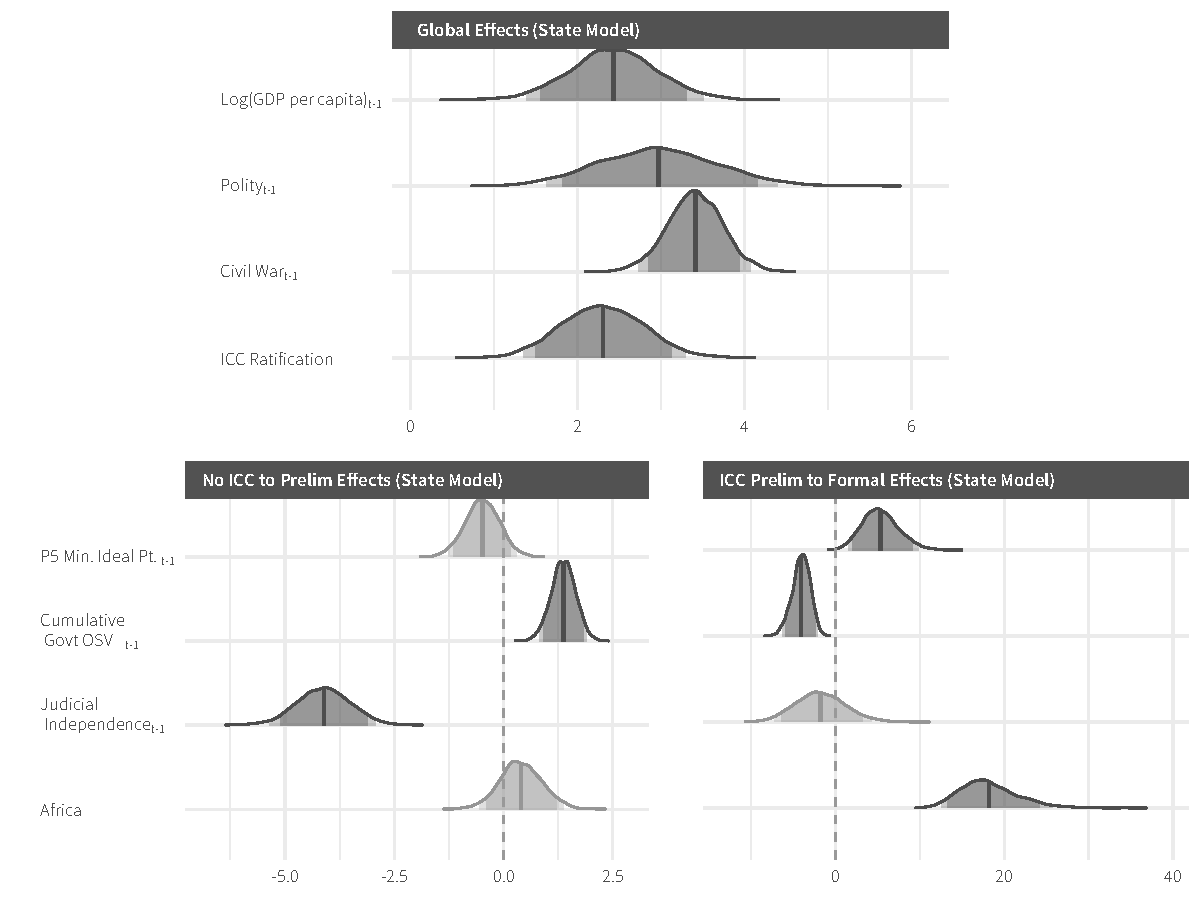
\includegraphics[width=1\textwidth]{stateCoefSumm.pdf}
    \caption{Parameter estimates from State-Focused ICC Transition model visualized through posterior distributions with median values designated by vertical line, lightly shaded portion indicating the 95\% credible interval, and darker shaded portion the 90\% credible interval.}
    \label{fig:stateModel}
\end{figure}

\begin{figure}
    \centering
    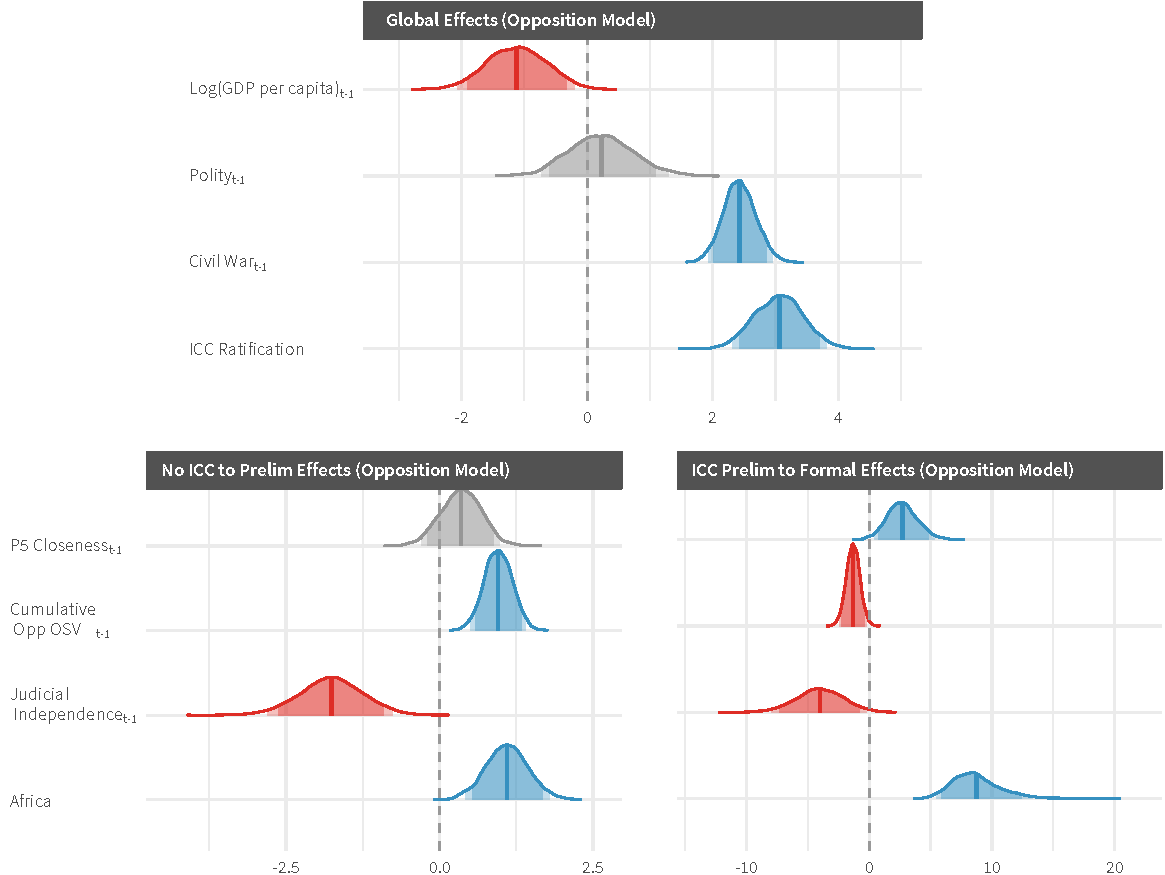
\includegraphics[width=1\textwidth]{rebelCoefSumm.pdf}
    \caption{Parameter estimates from Opposition-Focused ICC Transition model visualized through posterior distributions with median values designated by vertical line, lightly shaded portion indicating the 95\% credible interval, and darker shaded portion the 90\% credible interval.}
    \label{fig:rebelModel}
\end{figure}
% figure out a better way to depict results, since plots won't print in color - the grey vs blue vs red won't show up... right?

Figure \ref{fig:stateModel} presents the results for the transition to a \textit{government-targeted} preliminary examination and formal investigation. Figure \ref{fig:rebelModel} presents the results for \textit{opposition-targeted} preliminary examinations and formal investigations.
% add something here about what the figures present - standardized coefficient estimates with credible intervals? Something else? also add a sentence justifying standardized coefficients, and explain that they're useful for comparing size of effect across variables of interest.  I'm not sure what to say here - either Ben or SM can fill in.

Based on the logic of impartiality, we hypothesized that the OTP would be more likely to initiate a preliminary examination and advance to a formal investigation targeting a particular government when that government perpetrated more civilian targeting (H1), and that the OTP would be less likely to initiate examinations or advance to investigations against governments with more independent judiciaries (H2). The results in Figure \ref{fig:stateModel} demonstrate that the decision to initiate a preliminary examination (i.e. move from no ICC involvement to a preliminary examination) clearly follows the logic of impartiality. In line with H1, as the severity of government one-sided violence increases, the likelihood of the onset of a preliminary examination targeting that government also increases.  More substantively, the coefficient estimate for the OSV variable is 1.37, indicating that a one standard deviation increase in one-sided violence is associated with a 1.37 increase in the likelihood that the OTP initiates a preliminary examination against the government.
% i'm not clear on what units the 1.37 increase is.  a 1 standard deviation increase in OSV is associated with a 1.37 increase... what does this mean?  either add in % change info or take out the numbers altogether and just discuss how size of effect is larger/smaller than other key IVs (this goes for all similar comments below)

Similarly, in support of H2, increasing judicial independence reduces the likelihood that the OTP initiates a preliminary examination against the government. Thus, when considering the decision to initiate the first stage of ICC involvement against the government, the OTP's strategic decision-making does appear to be informed by the logic of impartiality. Interesting, the results suggest that this variable has a stronger substantive impact on OTP decision-making compared to the OSV measure. In particular, a one standard deviation increase in judicial independence is linked with a 4.12 decrease in the likelihood that the OTP starts a preliminary examination against the government. The judiciary variable also performs well compared to the other variables in the model; it has the largest substantive impact among the theoretical variables of interest and performs well against the global coefficients for the control variables.
% again unclear on the units for the size of effect 4.12 decrease

A similar picture emerges when considering the decision to initiate a preliminary examination targeting opposition actors. As Figure \ref{fig:rebelModel} demonstrates, increasing the level of one-sided violence perpetrated by opposition actors increases the likelihood that the OTP initiates a preliminary examination targeting the opposition, in line with H1. Specifically, we see that a one standard deviation increase in OSV is associated with a .96 increase in the likelihood that the OTP starts a preliminary examination against opposition actors.
% again question about units for the .96 increase

In line with the logic of impartiality, judicial independence again reduces the likelihood of the OTP initiating a preliminary examination in the opposition model.  Here, the coefficient estimate is -1.76, suggesting that a one standard deviation increase in the independent judiciary variable is associated with a 1.76 decrease in the likelihood of a preliminary examination targeting the opposition. Similar to the government model, the judiciary variable has the strongest substantive impact among the theoretical variables of interest.
% units for 1.76 decrease?

At the first stage, therefore, when the OTP must decide whether to initiate a preliminary examination, it appears that the logic of impartiality does influence her decision-making, whether crimes have been perpetrated by government or opposition actors. Furthermore, the result also suggest that complementarity, as proxied by an independent judiciary, has a strong impact on OTP decision-making, relative to the other theoretical variables of interest.

The OTP's incentive to adhere to the ICC's legal mandate, however, does not consistently extend to the decision to advance a situation to a formal investigation. While the logic of impartiality suggests that the OTP should prioritize the worst human rights abuses at both decision points, the results in Figure \ref{fig:stateModel} and Figure \ref{fig:rebelModel} indicate that the OTP is actually \textit{less} likely to advance from a preliminary examination to a formal investigation as abuses against civilian populations increase. While this negative effect seems surprising at first, we suspect that the OTP may be wary of advancing to an investigation in situations where the ability of the court's investigators to safely carry out their investigations and the security of witnesses may be compromised.\footnote{The deterrent effect of high OSV should be felt most at the second stage, when the OTP decides whether to initiate a formal investigation, as this stage requires a much greater OTP presence (i.e. investigators) on the ground.}

The effect of judicial independence is similarly weaker at the second stage. While more independent judiciaries reduce the likelihood of transition to formal investigations targeting opposition actors, as expected, judicial independence has no significant effect on the likelihood of moving from a preliminary examination to a formal investigation against government actors. %While more research is necessary to better understand the mixed results, it is possible that we observe a significant impact for judiciary only in the opposition model because governments may be more likely to prosecute members of the opposition than their own supporters to ward off a formal investigation.
%do you have any thought about why we find contradictory results.
% I'm not sure we want to make that point about why the effect doesn't hold in state model b/c it highlights that our measure is a pretty crappy proxy. I think its probably true that Judicial independence has no effect in the state model b/c it is probably associated with more trials against opposition than against state, and therefore OTP is still acting against states sometimes even when judiciary is independent.  but that just means our measure is bad. It suggests that the OTP could still be following the legal mandate, but we have no idea if that's true or not, since we don't directly measure complementarity.  We could just speculate more vaguely that more research is necessary to understand whether the null result is because the OTP's decision is less driven by complementarity in the second stage, or whether instead our measure needs further refinement. Not sure what the best strategy is.

Regarding the substantive impact in the opposition model, we see that a one standard deviation increase in judicial independence is associated with a 4.02 decrease in the likelihood that OTP moves to a formal investigation. Despite this significant result, it is nonetheless important to note that in the second stage,  we find no support for H1, and only mixed support for H2, suggesting that OTP decision-making is not primarily driven by the logic of impartiality in the second stage, when deciding whether to advance preliminary examinations to the formal investigation stage.

Unlike the logic of impartiality, the OTP's strategic incentives to consider P5 interests suggested that the OTP would target actors in states with weaker ties to the P5 when deciding whether to initiate a preliminary examination or advance to a formal investigation (H3). We again find mixed support for this argument. At the first stage, the OTP does not seem to be driven by incentives to prioritize P5 interests: distance from P5 states has no significant effect on the initiation of a preliminary examination in either the government (Figure \ref{fig:stateModel}) or opposition (Figure \ref{fig:rebelModel}) model. In other words, this result suggests that the OTP does not cater to powerful states' interests in an attempt to curry favor and increase their support for the court when deciding whether to open a preliminary examination targeting either government or opposition actors in a country.

At the second stage, on the other hand, P5 interests, as measured by ideal point distance, have a powerful effect on the OTP's decision-making. As demonstrated in Figures \ref{fig:stateModel} and \ref{fig:rebelModel}, the OTP is significantly more likely to advance a preliminary examination to the formal investigation stage against governments and opposition actors in states with weaker ties to powerful states (i.e. the P5). Substantively, we see that a one standard deviation increase in P5 ideal point distance is associated with a 5.5 and 5 increase in the onset of formal investigations in the government and opposition models, respectively.
% again, clarify unit of 5.5 and 5 increase.

The results for Africa are largely similar to those for the ideal point distance measure, as they vary across stages of ICC involvement. In the preliminary examination stage, Africa is only statistically significant in the opposition model. In particular, a one standard deviation increase is associated with a 1.10 increase in the likelihood that the OTP initiates a preliminary examination against opposition actors. Interestingly, the substantive impact of this variable is smaller than the other statistically significant variables and the the control variables. Thus, the relatively small substantive effect along with insignificant result in the government model raises important questions regarding the conventional wisdom of the so-called African bias, which claims that the OTP is always more likely to target Africans because of African states' relatively smaller geo-strategic importance to powerful states.
% again, clarify unit for the 1.1 increase for Africa in opposition model
% is the effect of Africa really smaller than OSV?  it doesn't look that way in the figure, but i might be wrong. can we say effect is smaller than the impartiality variables specifically, instead of saying "other significant variables"?  Again i'm also wary of comapring to the controls since those are global coefficients.

On the other hand, we find that Africa is associated with a higher probability of formal examinations in both the government and opposition models. Not surprisingly, this variable produces the largest substantive effect in the second stage, as the coefficient estimates are 18.19 and 8.74 in the government and opposition models, respectively. These results are also in line with the findings from the ideal point distance measure for P5 interests. Taken together, the results for Africa across the two stages of the two models reinforces the conclusion that the OTP's decision-making is affected by the interests of powerful states primarily at the second decision point, when deciding whether to advance a preliminary examination to the formal investigation stage. The results for Africa also speak to the claim that the OTP is biased against Africa: the OTP's tendency to favor African targets appears to be largely limited to the formal investigation stage.

Turning briefly to control variables, we find that they behave largely as expected across the models. As a reminder, we only assess the global effects of the controls due to sparse data. As expected, in both the government and opposition models, both civil war and ICC ratification are significantly associated with a higher probability of ICC involvement. The results for polity, on the other hand, do not match expectations: polity is insignificant in the opposition model, and is positive and significant in the government model. This unexpected positive result is likely driven by high-profile examinations of government actors in strongly democratic states, including the US, UK, and Israel. We also see mixed results for GDP per capita; the measure is positive and significant in the government model, while it is negative and significant in the opposition model. While this result requires more research, it is not entirely surprising, given that we anticipated that economic development could affect OTP involvement in different ways with contradictory effects.
% Ben, is what I said about democracy result OK?

% add paragraph here about model fit and comparison to ologit, selection model, etc. demonstrate that our model produces better and different results (assuming that's true).  we probably also need to think about selection type models, and why we don't use those (or how our results are better than if we used those, since the selection process is kind of obvious here and IR people will think that's an obvious modeling strategy, moreso than ologit probably)


\section*{Conclusion}

The ICC is a novel institution with the authority to investigate and prosecute individuals suspected of committing grave violations of international law.  Despite a burgeoning literature on the Court, scholars have neglected to systematically investigate when the Court becomes involved in a situation.  This paper attempts to fill this important gap in the literature. To that end, we put forward two theoretical arguments to explain why the Court initiates a preliminary examination in a state and whether it escalates its involvement.  Specifically, we first posited that the Court acts in accordance with its mandate and thus it is more likely to become involved in states with gross violations of human rights. We second argued that the Court’s behavior follows more of a realist logic, hypothesizing that the ICC is less likely to become involved or escalate its involvement when P5 interests are at stake. 

A series of empirical tests provide important insights into the applicability of each of these theoretical arguments to the behavior of the Court. First, we find fairly consistent support for most of our legal framework variables, suggesting that the law and institutional incentives help to explain when the Court becomes involved in a situation. We also observe some interesting results for the independent judiciary variable. The results indicate that complementarity is most likely to matter when it comes to the decision to escalate ICC involvement.  P5 interests also play an important role, particularly in the Court’s decision to escalate its involvement beyond the preliminary examination stage.  Close military ties with members of the P5, as well as political/policy affinity, influence the ICC’s willingness to advance its involvement in a given state.  Finally, we also find some important results regarding the relationship between Africa and the Court.  The ICC’s so-called Africa problem is more complex than much existing commentary indicates. We find no evidence to suggest that the Court singles out Africa when it starts preliminary examinations. However, consistent with some critics, we find that the Court has clearly chosen to focus on situations in Africa when it comes to formal investigations, warrants, and trials. 	

The argument advanced and the empirical results have important implications for both scholars and researchers interested in the ICC and human rights more generally.  We find support for both our legal mandate and institutional constraints arguments, suggesting that the Court’s decision-making is complex. Scholars debate whether international bodies are really independent or whether they simply reflect the interests of powerful states. Our analysis of the ICC, one of the most independent international institutions, suggests that even this organization cannot fully divorce itself from the influence of powerful states.  In its quest for institutional legitimacy, the ICC must serve the dual goals of fulfilling its mandate and remaining cognizant of powerful states’ interests. Finally, we address the so-called Africa bias in the Court and find mixed support for such claims.  Our findings suggest that the critics may overstate this problem to some extent, but that some bias does exist. 


\renewcommand{\thefigure}{A\arabic{figure}}
\setcounter{figure}{0}
\renewcommand{\thetable}{A.\arabic{table}}
\setcounter{table}{0}
\renewcommand{\thesection}{A.\arabic{section}}
\setcounter{section}{0}

\section*{Appendix}

\subsection*{Model Layout}

\begin{align*}
  Likelihood:& \\
  Y_{i} &\sim Continuation-Ratio(\mu_{i}, \tau_{k}) \\
  Linear Model:& \\
  \mu_{i} &= X_{i} \beta + W_{i}\eta_{k} + \alpha_{j}[i] \\
  Priors:& \\
  \beta_{p} &\sim T(0, 10, 3), \text{ for } p = 1, \ldots p \\
  \eta_{qk} &\sim T(0, 10, 3), \text{ for } q = 1, \ldots Q \text{ and } k =1, \ldots, K-1 \\
  \tau_{k} &\sim N(0, 1.5), \text{ for } k = 1, \ldots, K-1 \\
  \alpha_{j} &\sim N(0, \sigma_{\alpha}) \\
  Hyperpriors:& \\
  \sigma_{\alpha} &\sim Exponential(2)
\end{align*}

To describe our model we use the convention in \citet{mcelreath2016statistical}. The first two lines describe the likelihood and linear model and the remaining define the prior distribution for each parameter in the model. Let $Y_{i}$ be a particular country-year observation's score on our dependent variables. Both of our dependent variables take an integer value of $k=1, \ldots, K$. The framework we presented in our paper treats $Y_{i}$ as a function of a normally-distributed latent variable with a mean of $\mu$ and a standard deviation of 1. The $k=1, \ldots, K-1$ threshold parameters, $\tau$, partition this distribution into $K$ sections. The area of each of these sections describe the probability of falling into each response category.

To model changes in these probabilities, the models assume $\mu$ to be an additive combination of linear effects. We parameterize this model via first a set of variables, $X$ that are thought to effect the probability of falling into a particular category equally and the effect of these variables is captured by a $P$ length vector of coefficients, $\beta$. We also include $Q$ variables that have category specific effects and these are denoted by $W$ and their effect is measured by $\eta$. $\alpha$ represents a set of varying effects that account for country-ICC case specific unmeasured variation.

For both the \emph{State- and Opposition-Focused ICC Transition} models we utilize the same set of prior distributions. For $\beta$ and $\eta$ we use Student's t priors with three degrees of freedom. For the threshold parameters, $\tau$, we use a Normal distribution with a mean of zero and standard deviation of 1.5. We also use normally distributed priors for $\alpha$ and set the mean to zero and standard deviation to $\sigma_{\alpha}$, which  has its own Exponential hyperprior with a rate of 2.

\subsection*{Convergence Check for Main Models}

Below we show trace plots, after a burn-in period of 4,000 iterations, for both the \emph{State- and Opposition-Focused ICC Transition} dependent varibales. In both cases, we can see that the chains seem to be mixing well and have converged.

\begin{figure}
    \centering
    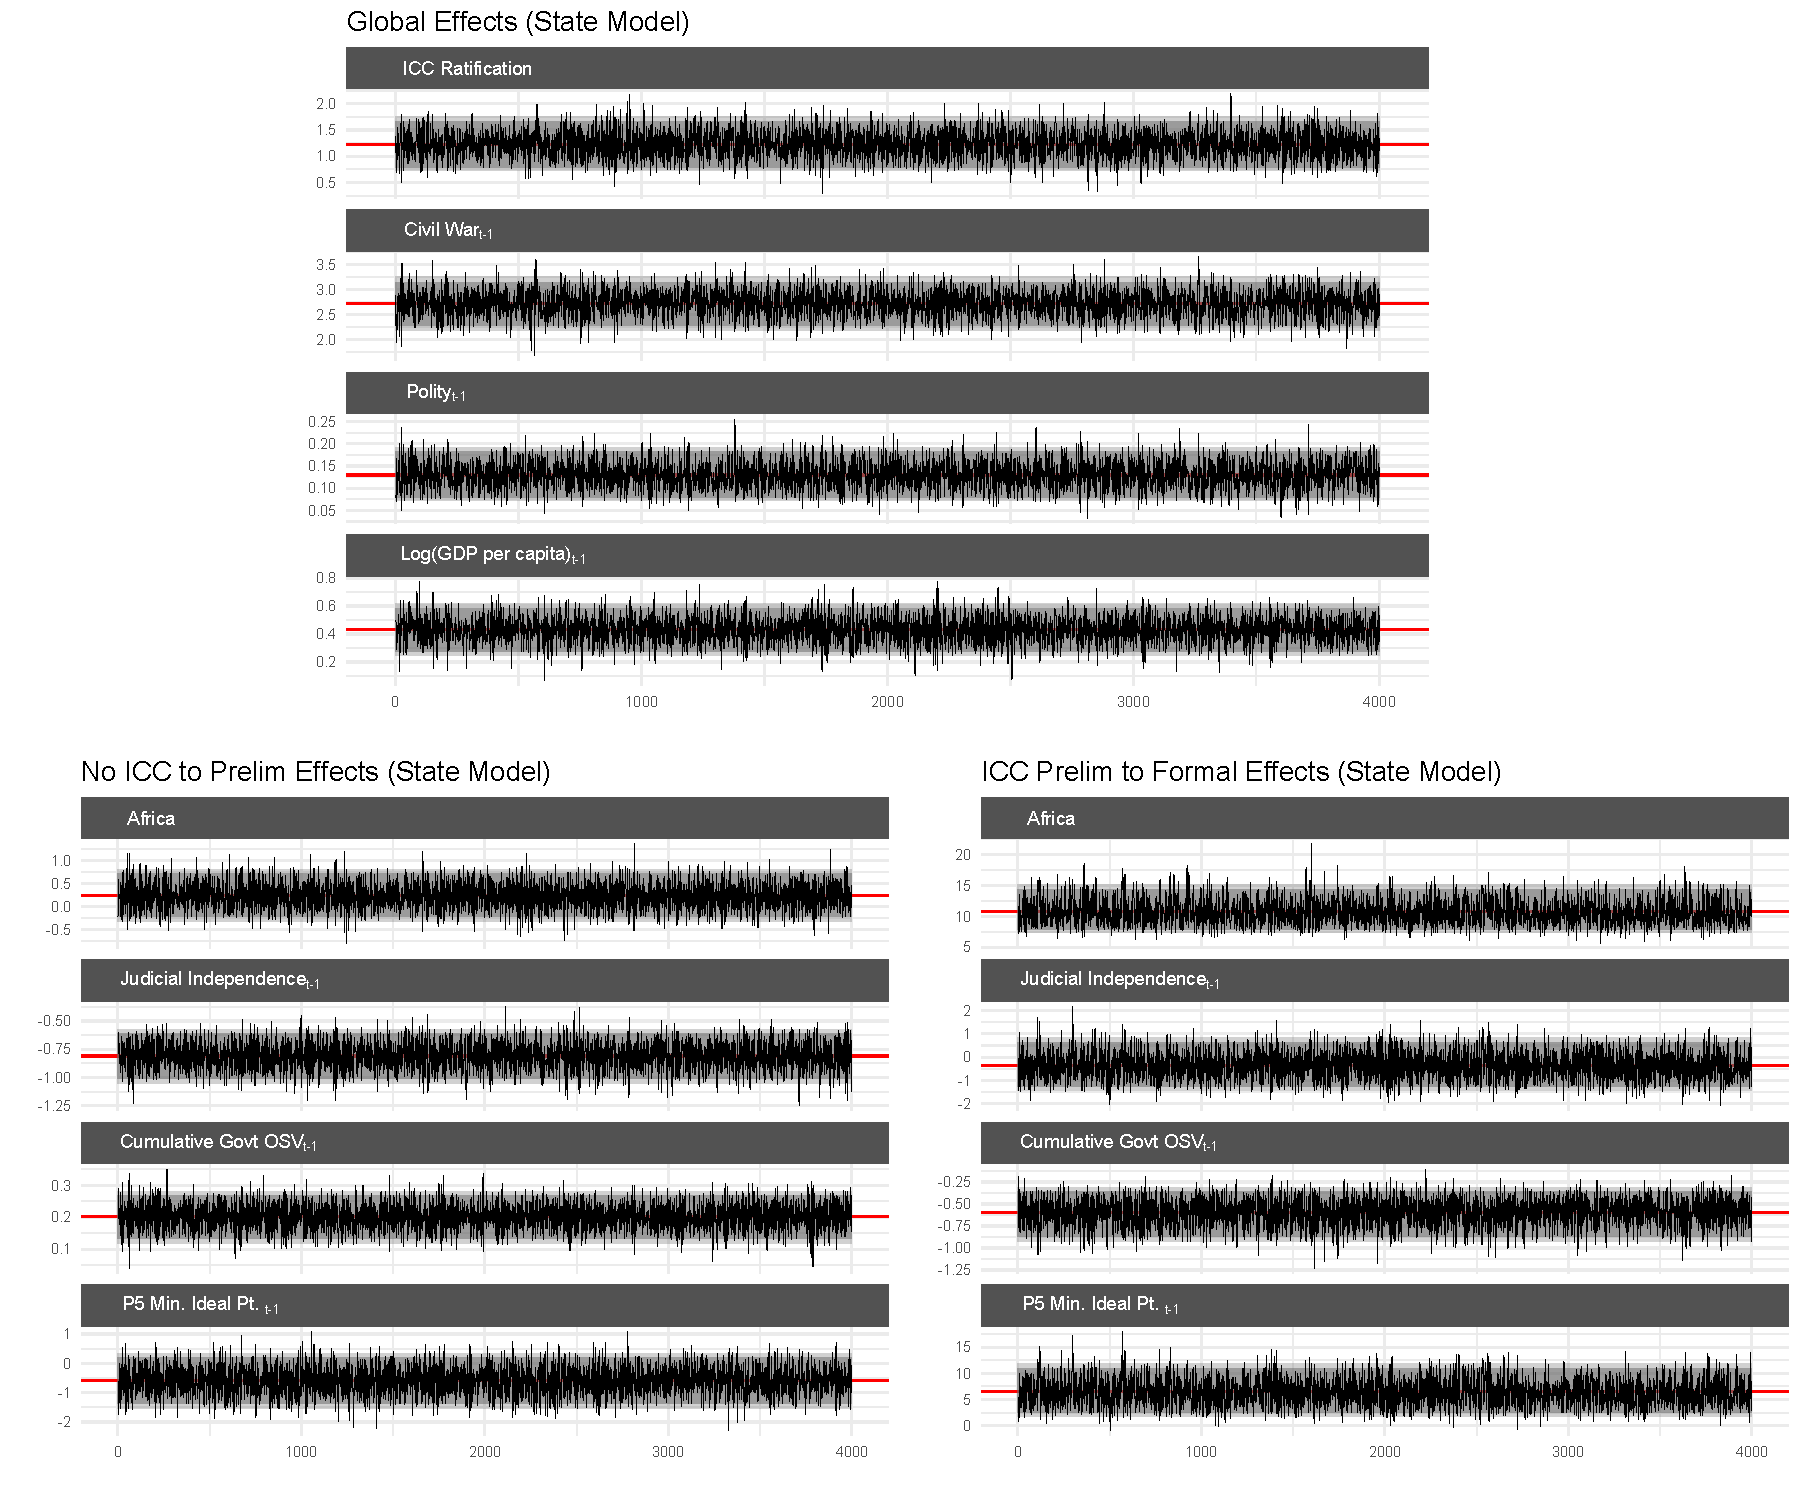
\includegraphics[width=1\textwidth]{stateCoefTrace.pdf}
    \caption{Trace plot for \emph{State-Focused ICC Transition} model.}
    \label{fig:stateTrace}
\end{figure}
\FloatBarrier

\begin{figure}
    \centering
    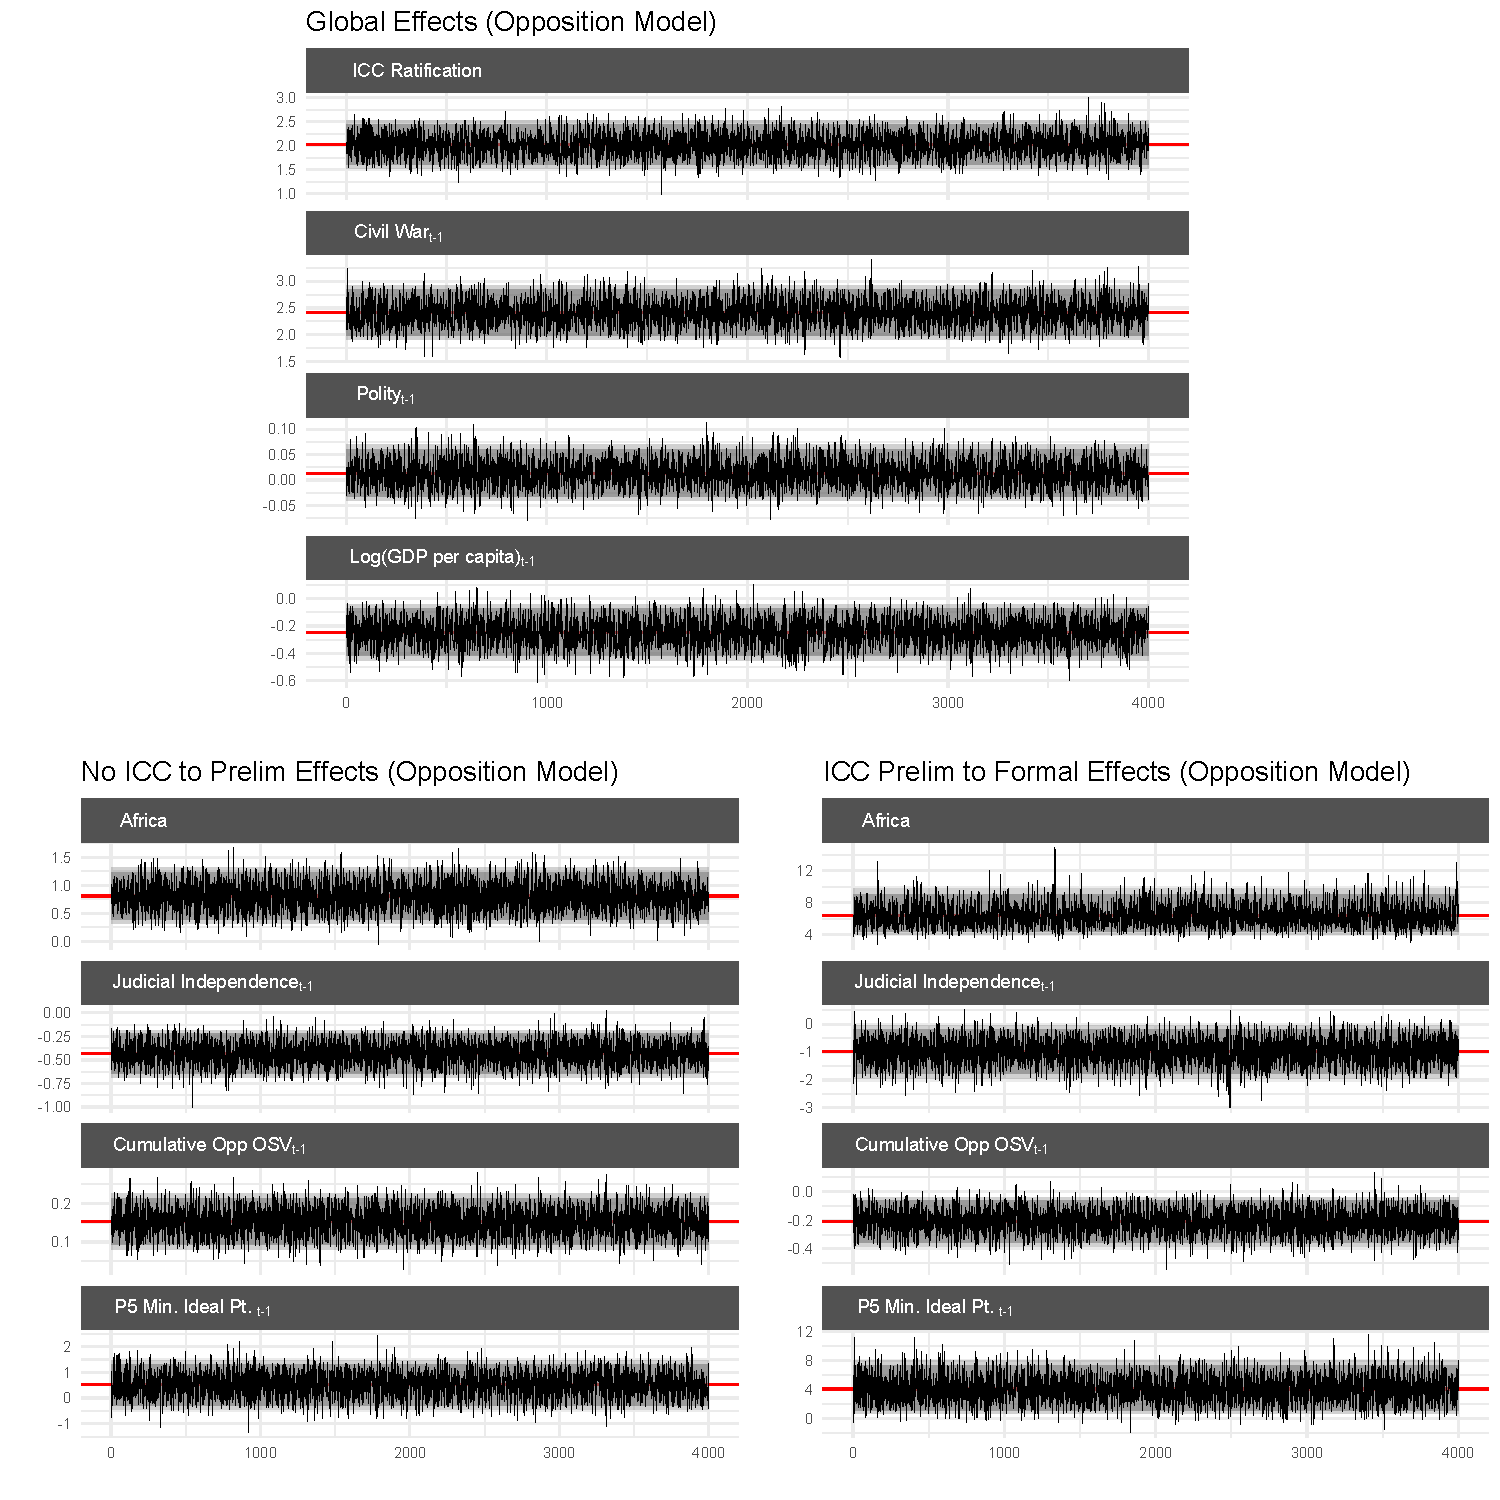
\includegraphics[width=1\textwidth]{rebelCoefTrace.pdf}
    \caption{Trace plot for \emph{Opposition-Focused ICC Transition} model.}
    \label{fig:oppTrace}
\end{figure}
\FloatBarrier

\subsection*{PTS \& ICC Ratifier Robustness Check}

% pts greather than 3 andd icc ratif equals 1

We examine the robustness of our results to a sample restriction. Specifically, we subset our sample to those cases where the PTS value is greater than three and only ICC ratifiers. Results are shown below and are broadly similar to what we report in the paper.

\begin{figure}
    \centering
    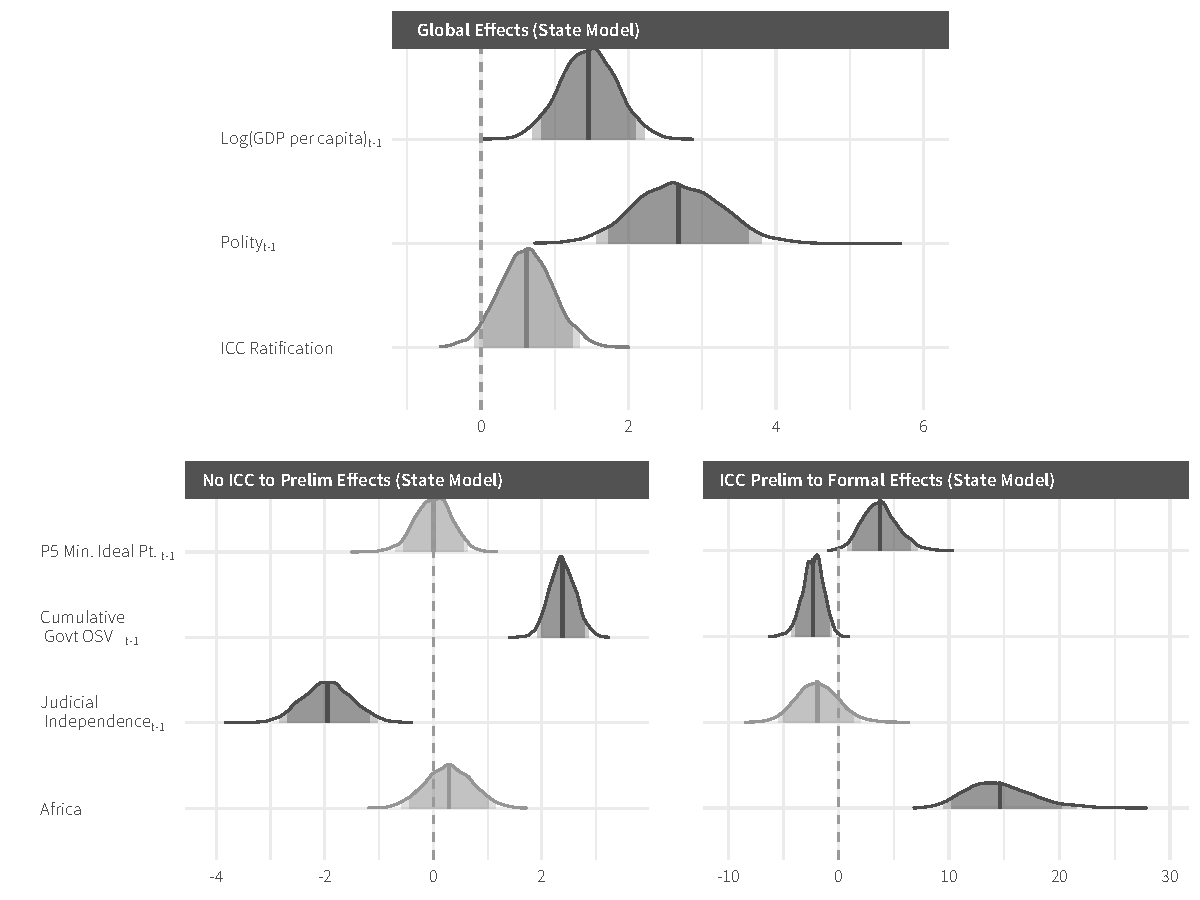
\includegraphics[width=1\textwidth]{stateCoefSumm_ptsCivilWarOnly.pdf}
    \caption{Parameter estimates when restricting sample to PTS greater than three and only ICC ratifiers from State-Focused ICC Transition model visualized through posterior distributions with median values designated by vertical line, lightly shaded portion indicating the 95\% credible interval, and darker shaded portion the 90\% credible interval.}
    \label{fig:stateModel_pts3_icc1}
\end{figure}

\begin{figure}
    \centering
    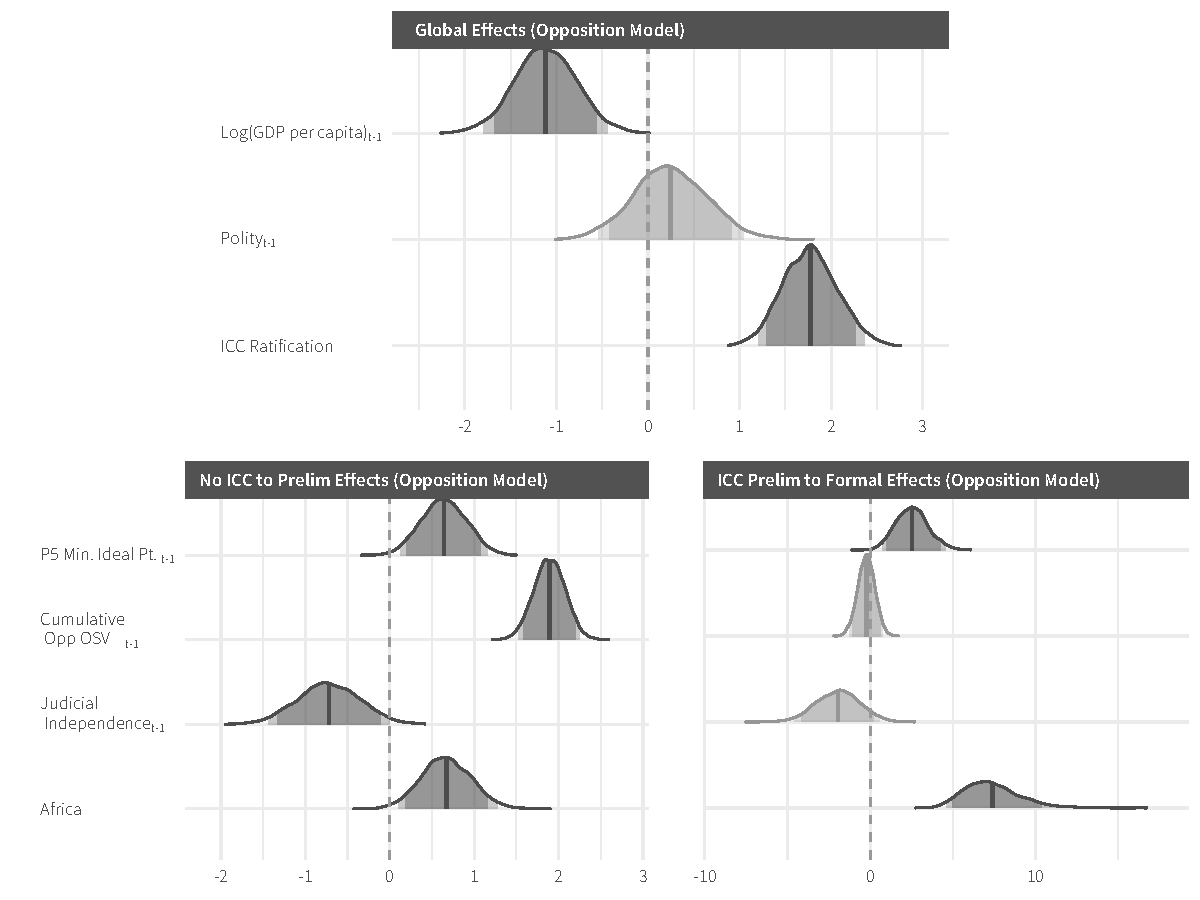
\includegraphics[width=1\textwidth]{rebelCoefSumm_ptsCivilWarOnly.pdf}
    \caption{Parameter estimates  when restricting sample to PTS greater than three and only ICC ratifiers from Opposition-Focused ICC Transition model visualized through posterior distributions with median values designated by vertical line, lightly shaded portion indicating the 95\% credible interval, and darker shaded portion the 90\% credible interval.}
    \label{fig:rebelModel_pts3_icc1}
\end{figure}

\subsection*{Results without imputation}

To make sure that our results are not being driven by our multiple imputation procedure we also run a version of our sampler in which we employ listwise deletion. The results are shown below and are broadly similar to those reported in the paper.

% Results broadly the same ... p5min ideal point in no icc to prelim eff same direction but no longer sig, africa in no icc to prelim same direction but no longer sig ... everything else the same

\begin{figure}
    \centering
    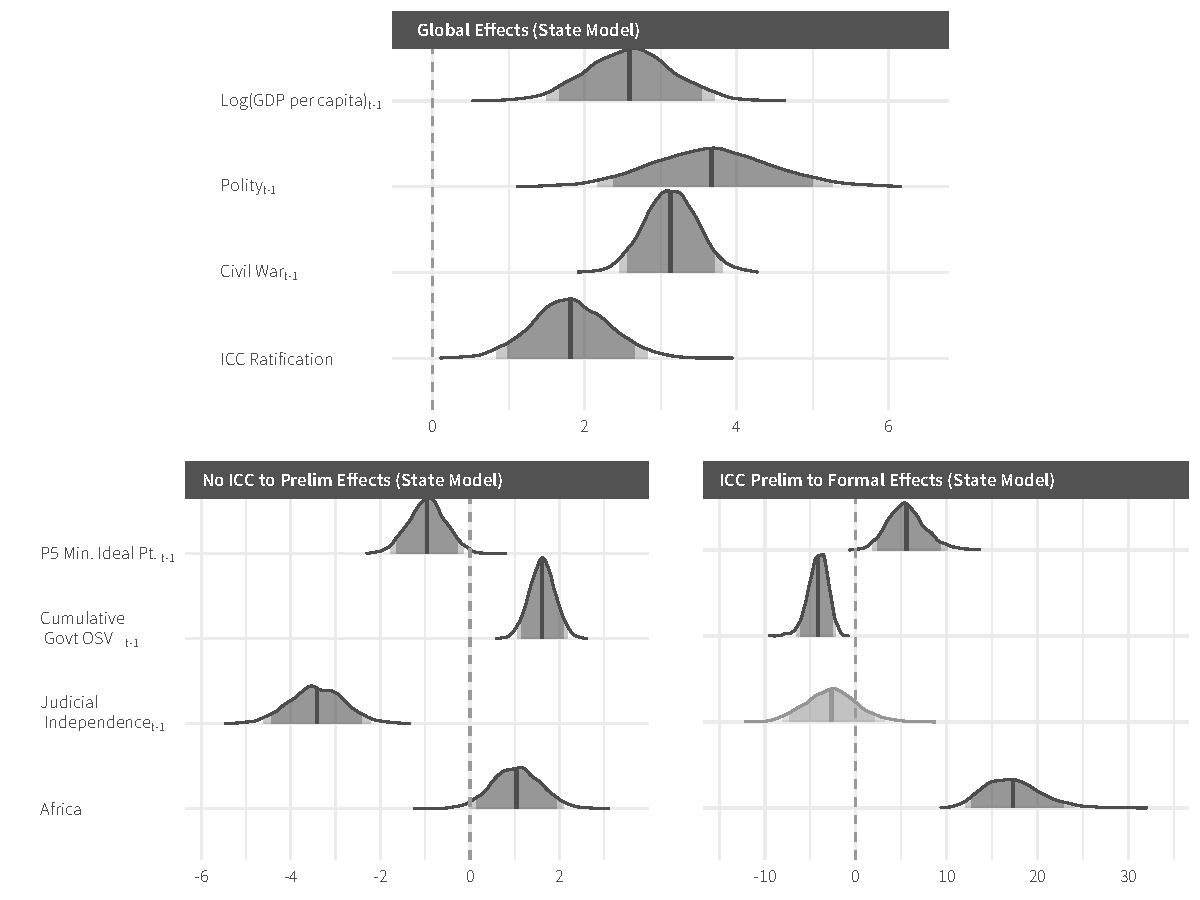
\includegraphics[width=1\textwidth]{stateCoefSumm_noImp.pdf}
    \caption{Parameter estimates when using listwise deletion from State-Focused ICC Transition model visualized through posterior distributions with median values designated by vertical line, lightly shaded portion indicating the 95\% credible interval, and darker shaded portion the 90\% credible interval.}
    \label{fig:stateModel_noImp}
\end{figure}

% Results broadly the same ... evidence stronger for cumm opp osv in icc prelim to formal effects

\begin{figure}
    \centering
    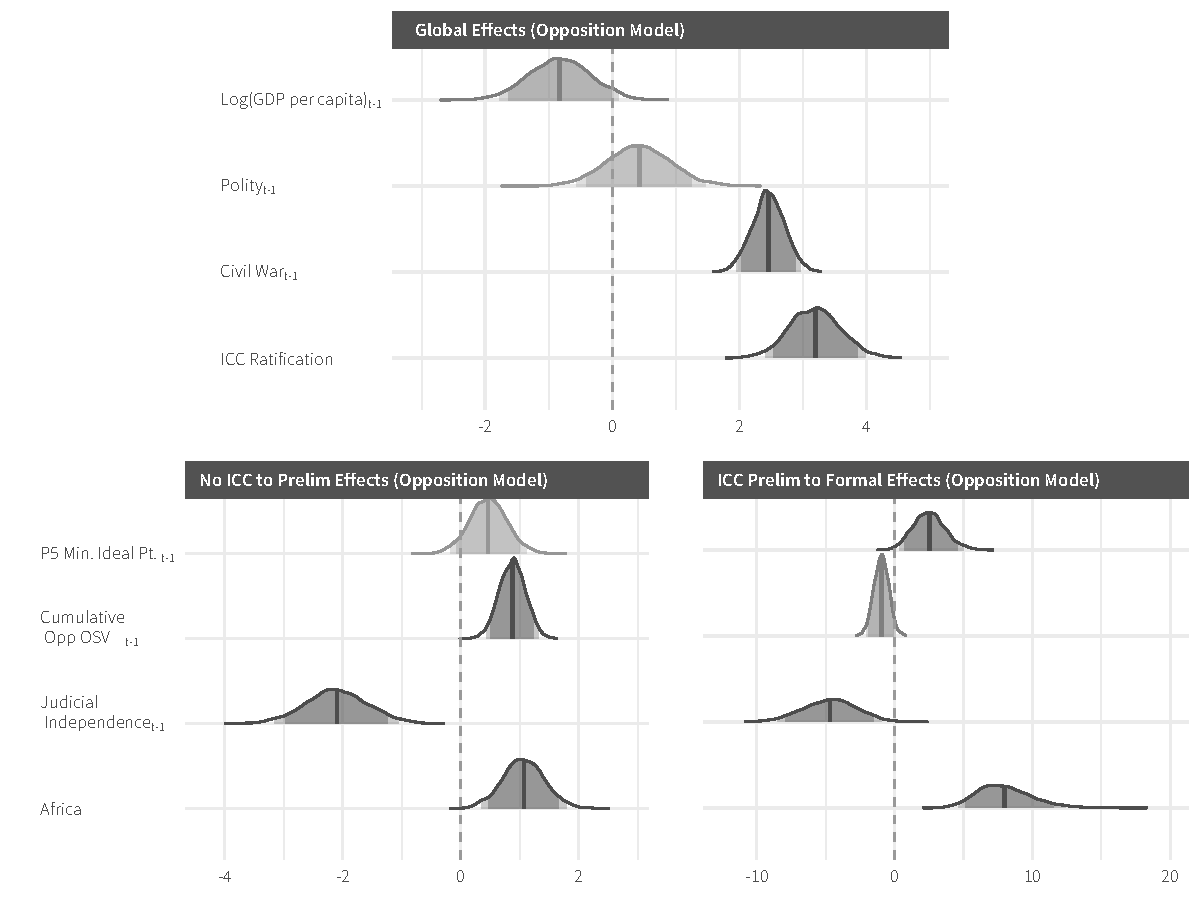
\includegraphics[width=1\textwidth]{rebelCoefSumm_noImp.pdf}
    \caption{Parameter estimates when using listwise deletion from Opposition-Focused ICC Transition model visualized through posterior distributions with median values designated by vertical line, lightly shaded portion indicating the 95\% credible interval, and darker shaded portion the 90\% credible interval.}
    \label{fig:rebelModel_noImp}
\end{figure}

\subsection*{Comparison with ordinal logit}

To show the utility of our approach we also compare it against

\begin{figure}
    \centering
    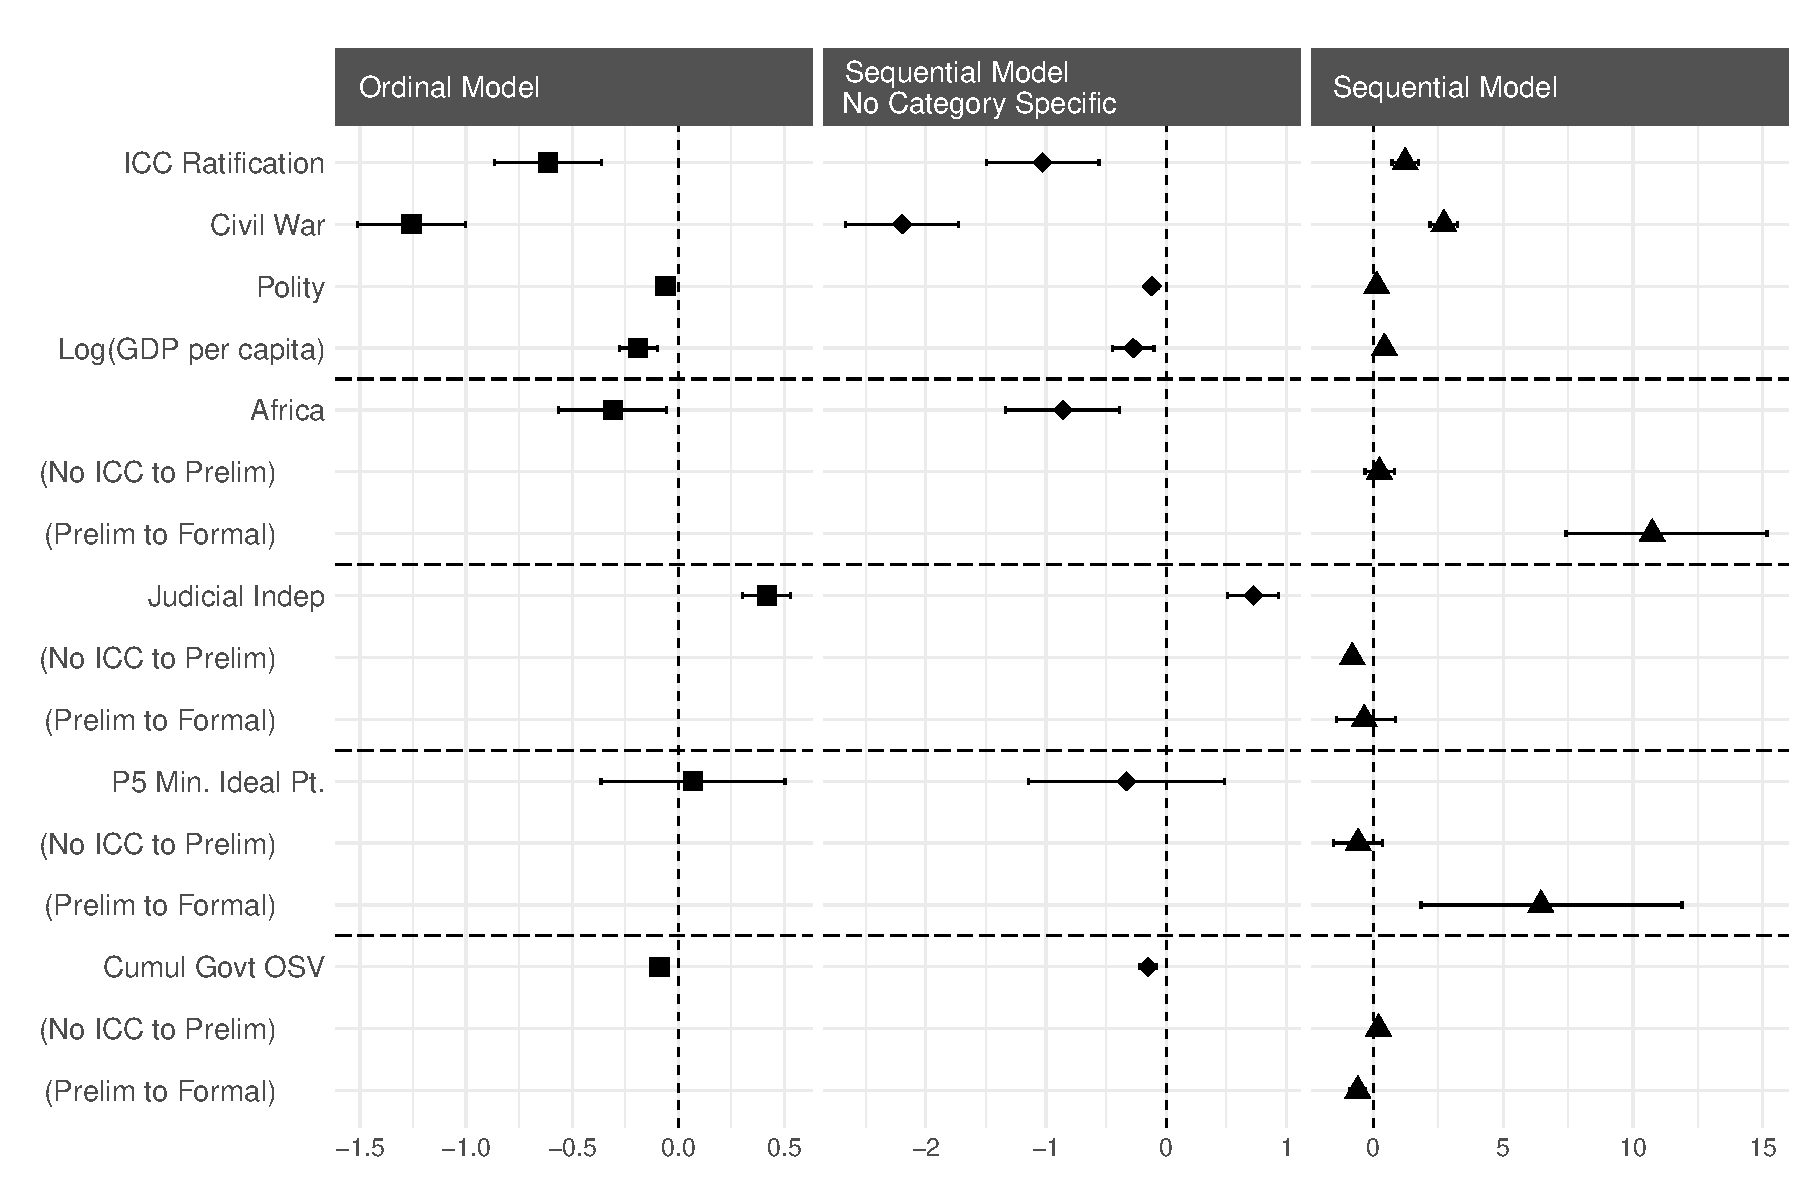
\includegraphics[width=1\textwidth]{modCompare_state.pdf}
    \caption{State model.}
    \label{fig:stateCoefCompare}
\end{figure}

\begin{figure}
    \centering
    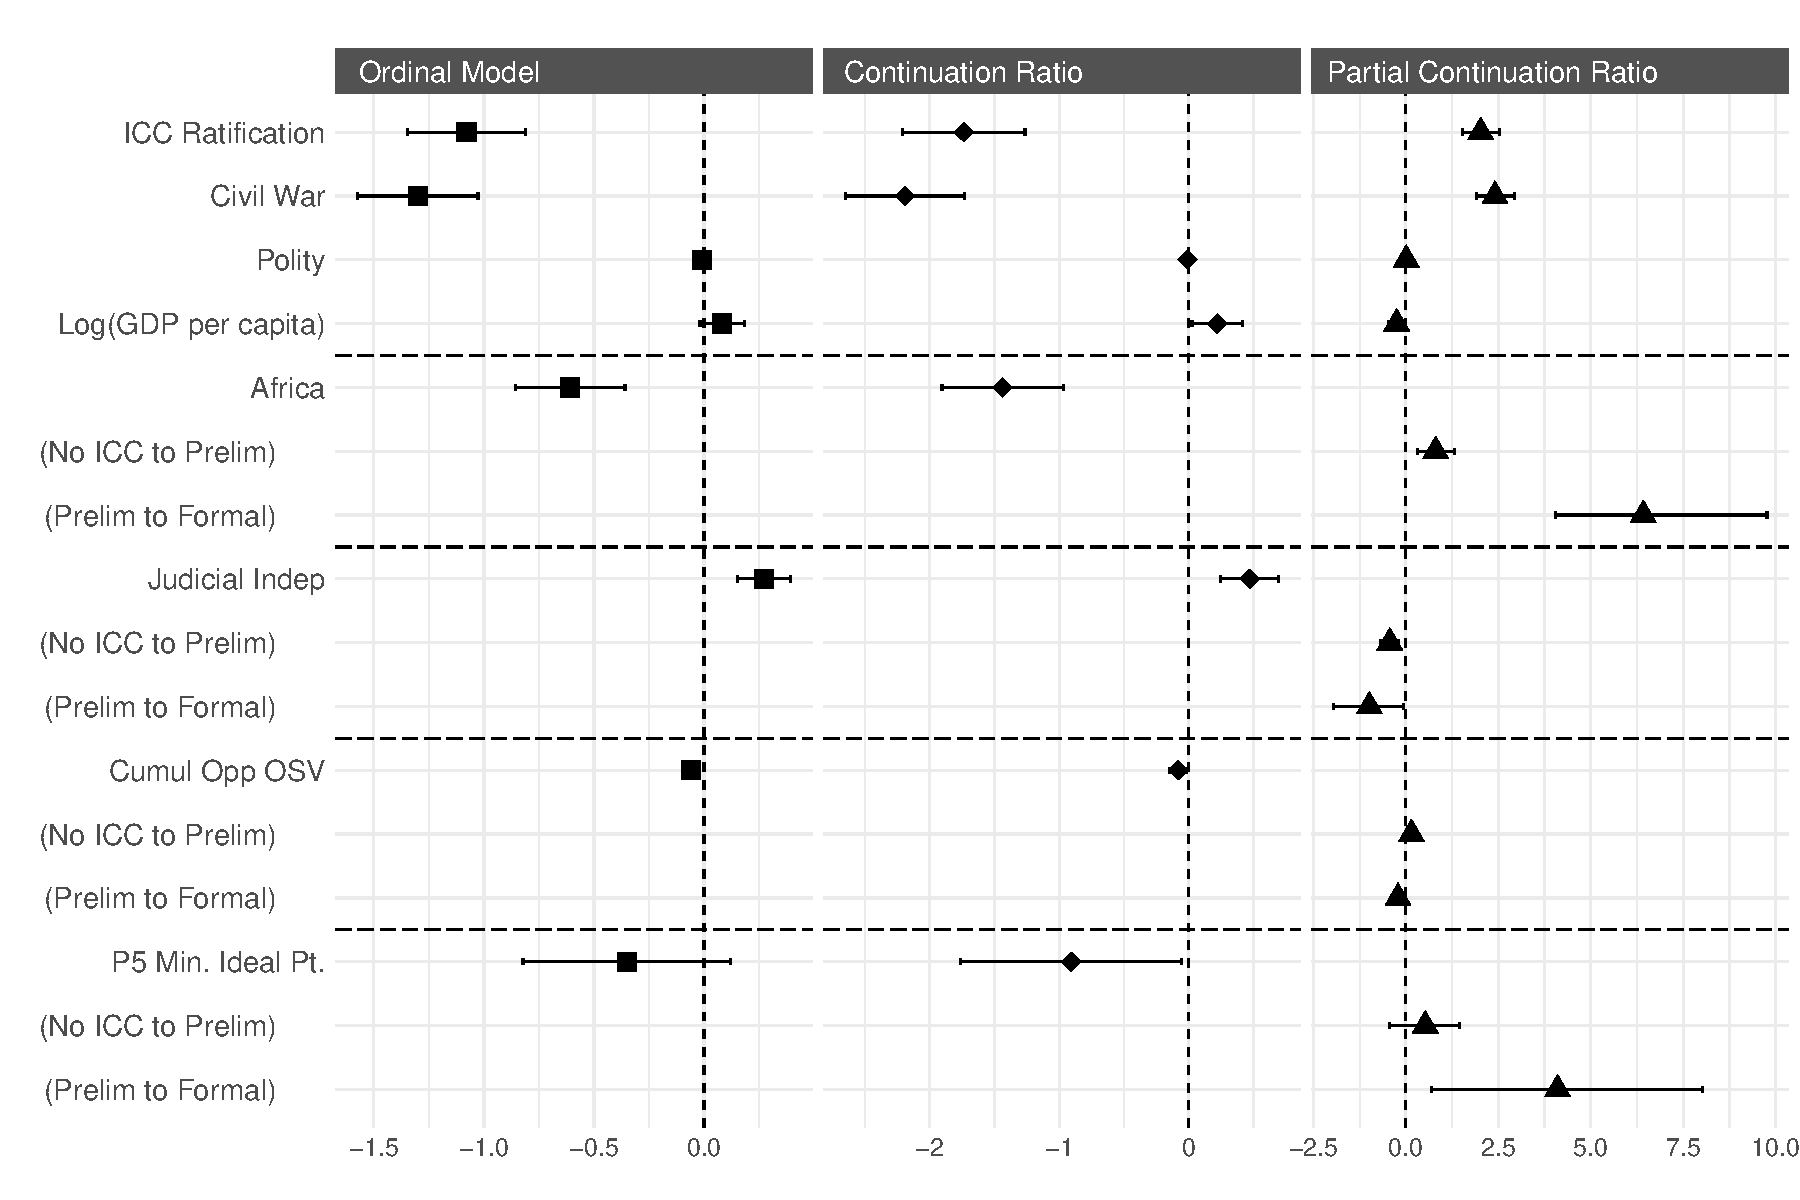
\includegraphics[width=1\textwidth]{modCompare_opp.pdf}
    \caption{Opposition model.}
    \label{fig:oppCoefCompare}
\end{figure}

For ordinal variables the choice of a fit statistic is not as obvious. We use Somer's $D$, a rank correlation coefficient  \citep{Somers1962}, as our discrepancy statistic for the ordinal logit models. Somer's $D$ is closely related to Goodman and Kruskal's $\gamma$ and Kendall's $\tau$, differing only in the denominator.\footnote{Somer's $D$ is similar to the commonly used $\tau_b$, which is equal to $\frac{P - Q}{(P+Q+X_0)(P+Q+Y_0)}$, where $Y_0$ is the number of ties in $Y$, and $\gamma$, which is equal to $\frac{P - Q}{P + Q}$.} Somer's $D$ makes a distinction between the independent and dependent variable in a bivariate distribution, correcting for ties within the independent variable. With $Y$ being treated as the independent variable it is denoted $D_{xy}$.

Specifically:
$$D_{xy} = \frac{P - Q}{P + Q + X_0}$$

\noindent where $P$ is the number of concordant pairs, $Q$ is the number discordant pairs, and $X_0$ is the number of ties in $X$. This is simply a measure of association for ordinal variables, so our approach is essentially to calculate the correlation between predicted and observed values. Like all correlation coefficients, the $D$ statistic lies in the interval $[-1, 1]$, with values closer to $1$ indicating more rank agreement and values closer to $1$ indicated less rank agreement, so values closer to 0 indicate more prediction error.

\begin{figure}
    \centering
    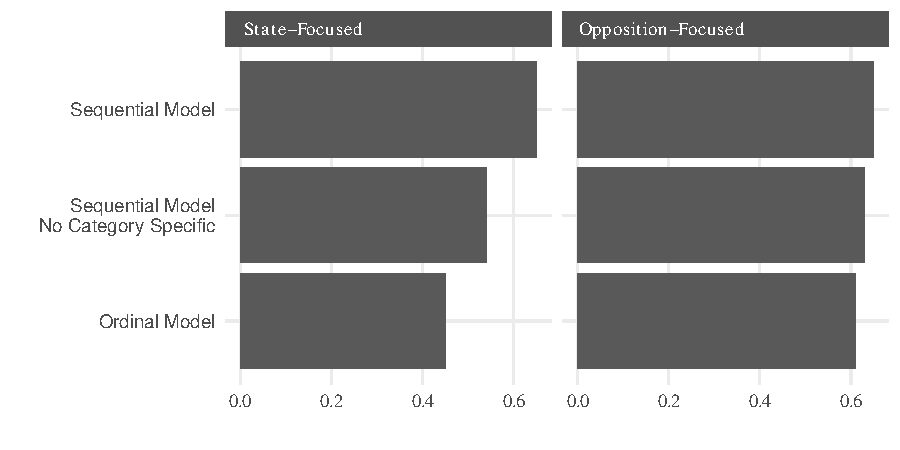
\includegraphics[width=1\textwidth]{somerViz.pdf}
    \caption{Performance comparison.}
    \label{fig:somersD}
\end{figure}


% Bib stuff
\clearpage
% \singlespacing
\bibliography{iccBib}

% \bibliographystyle{elsarticle-harv}\biboptions{authoryear}
\bibliographystyle{apsr}

\end{document}
